%\clearpage  %%% Appendix를 새 페이지에서 시작
\appendix
\renewcommand{\thesection}{\Alph{section}} %%% TOC에 appendix numbering 재설정
\renewcommand{\thesubsection}{\arabic{subsection}}
\renewcommand{\thesubsubsection}{\arabic{subsubsection}}
\titleformat{\section}[hang] {\normalfont\fontsize{21}{21}\selectfont\bfseries}{\Alph{section}.}{1em}{} %%% Appendix section title의 재설정
\titleformat{\subsection}[hang] {\normalfont\fontsize{16}{16}\selectfont\bfseries}{\Alph{section}.\arabic{subsection}.}{1em}{}
\titleformat{\subsubsection}[hang] {\normalfont\fontsize{14}{14}\selectfont}{\Alph{section}.\arabic{subsection}.\arabic{subsubsection}.}{1em}{}
\titleformat{\paragraph}[hang] {\normalfont\fontsize{12}{12}\selectfont\it}{}{1em}{}
\renewcommand{\theequation}{\thesection.\arabic{equation}} %%% Appendix equation numbering 의 재설정
\renewcommand{\thefigure}{\thesection-\arabic{figure}} %%% Appendix figure numbering 의 재설정
\renewcommand{\thetable}{\thesection-\arabic{table}} %%% Appendix table numbering 의 재설정
\setcounter{equation}{0} %%% Appendix equation starting number의 초기화
\setcounter{figure}{0} %%% Appendix figure starting number의 초기화
\setcounter{table}{0} %%% Appendix table starting number의 초기화


\section{Arduino Code for Wave Maker}

% \subsection*{main.ino}
\lstinputlisting[language=c++]{wavemaker/a_pagefunc.ino}
\lstinputlisting[language=c++]{wavemaker/b_button.ino}
\lstinputlisting[language=c++]{wavemaker/c_move.ino}
\lstinputlisting[language=c++]{wavemaker/d_menu.ino}
\lstinputlisting[language=c++]{wavemaker/menu.ino}
\lstinputlisting[language=c++]{wavemaker/sin_wave.ino}

\section{Experiment Data}
\begin{quote}
    \textbf{Notice}: Graphs of the plate displacement and wave height over time were provided below. Units were omitted, which were $\mathrm{~rad/s}$ and $\mathrm{~cm}$ for $\omega$ and $A$, respectively. Out of the conditions given in the Method section, the following cases were omitted: $(\omega, ~A) = (3, 6), (3, 7), (3, 8), (3, 9), (3, 10), (4, 8), (4, 9), (4, 10)$

    Analyzing the data at such a low $\omega$ was meaningless since external noise was not negligible. Also, the motor moved unexpectedly with the cases of $\omega=4$ above, and they were not analyzed.
\end{quote}

\subsection{Plate movement}
\begin{figure}[H]
\begin{center}
\begin{tabular}{cc}
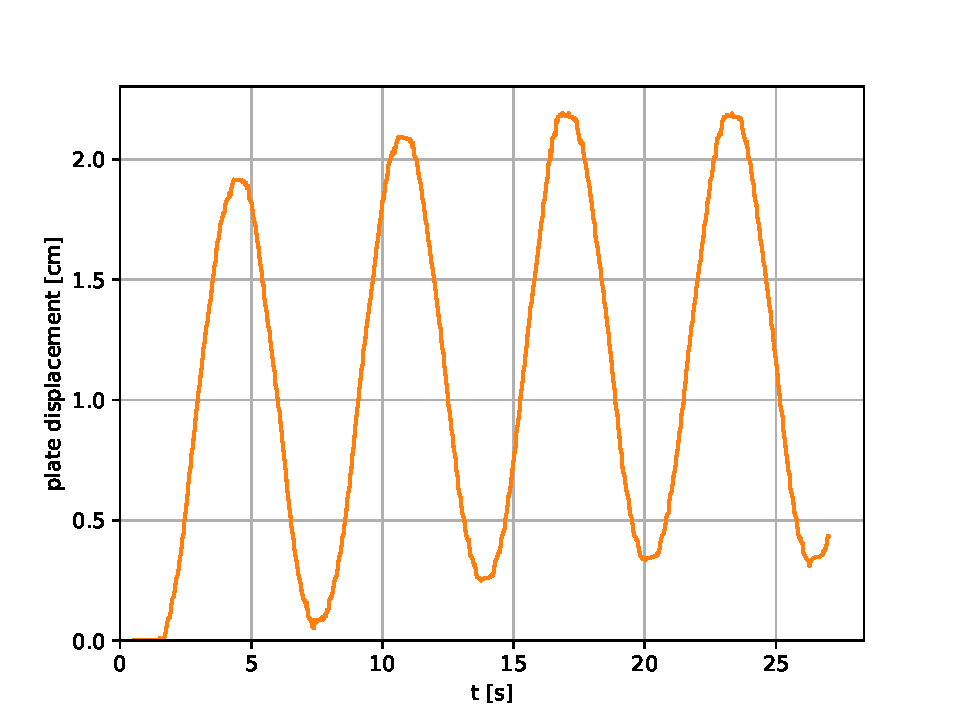
\includegraphics[width=0.45\textwidth, height=3.5cm]{graph/omega=0.50_A=1_plate.pdf}
&
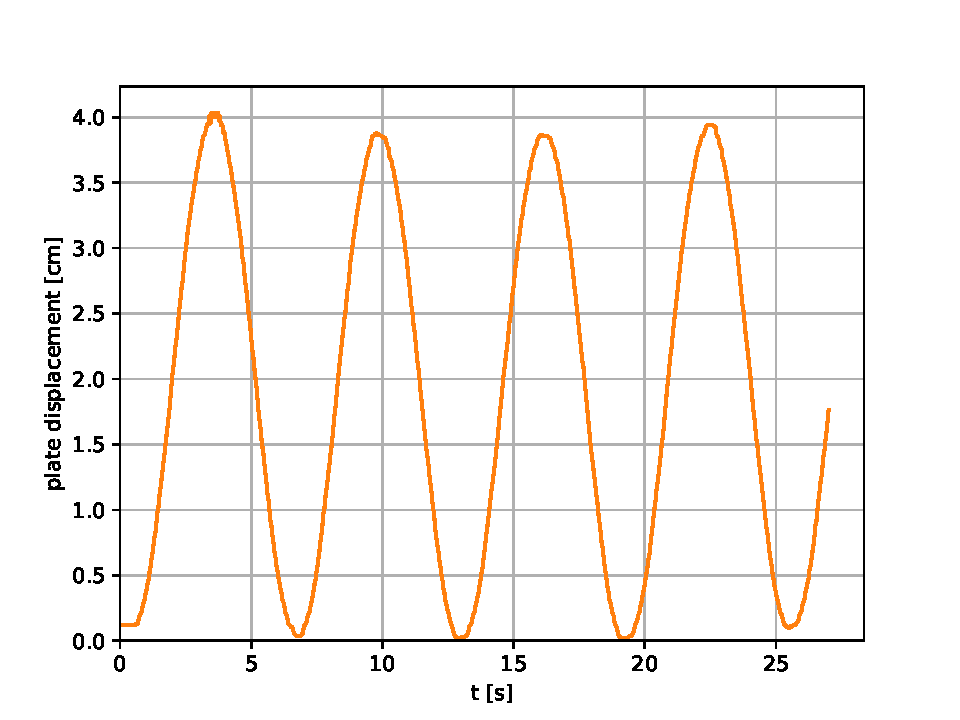
\includegraphics[width=0.45\textwidth, height=3.5cm]{graph/omega=0.50_A=2_plate.pdf}\\
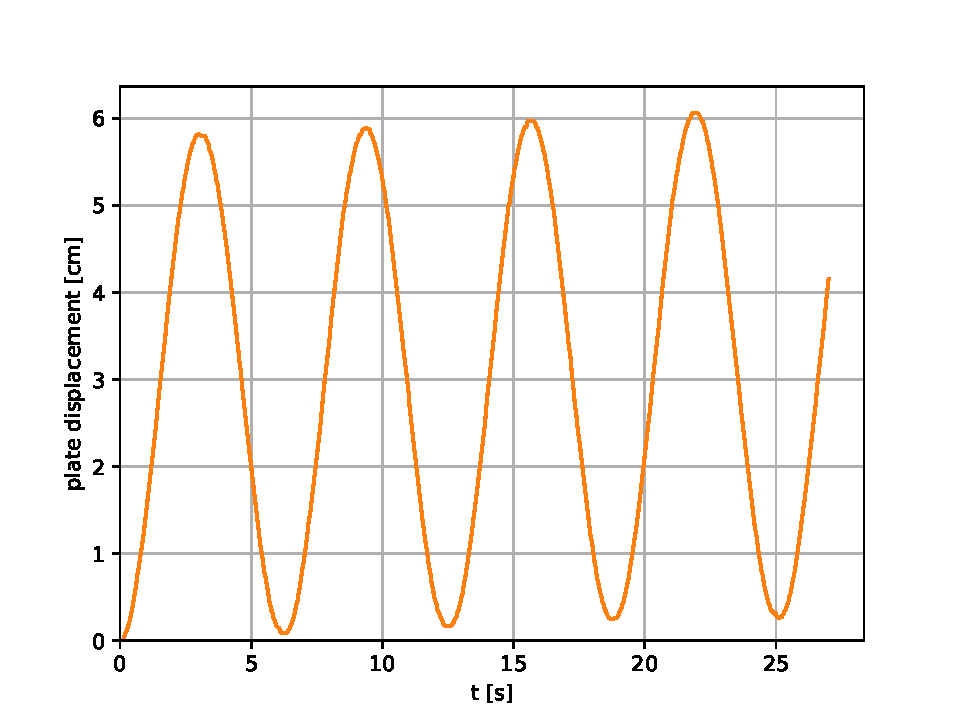
\includegraphics[width=0.45\textwidth, height=3.5cm]{graph/omega=0.50_A=3_plate.pdf}
&
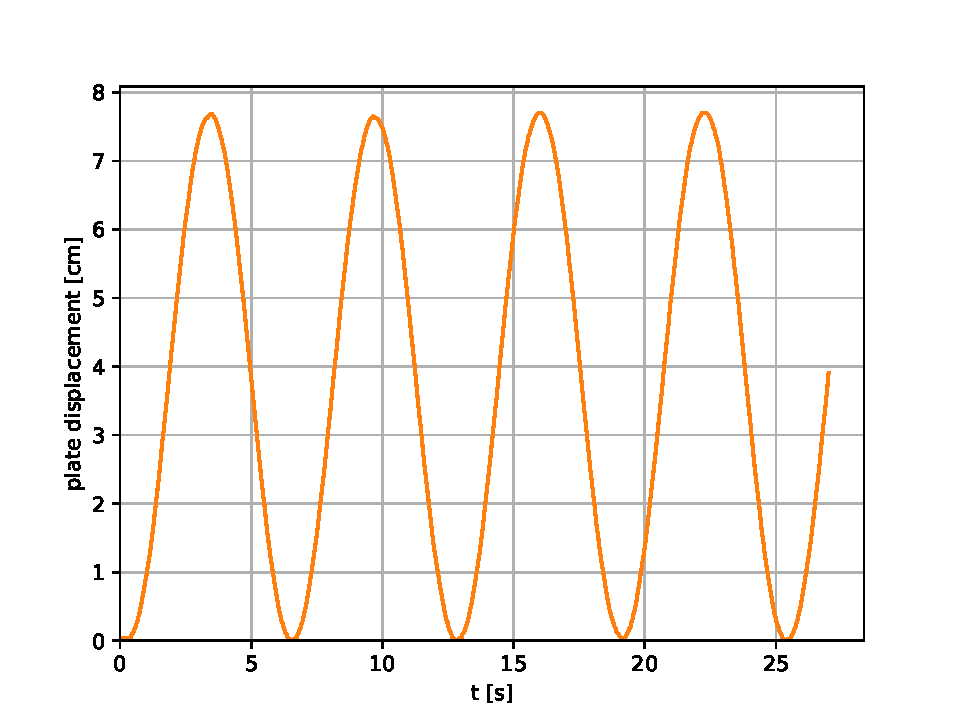
\includegraphics[width=0.45\textwidth, height=3.5cm]{graph/omega=0.50_A=4_plate.pdf}\\
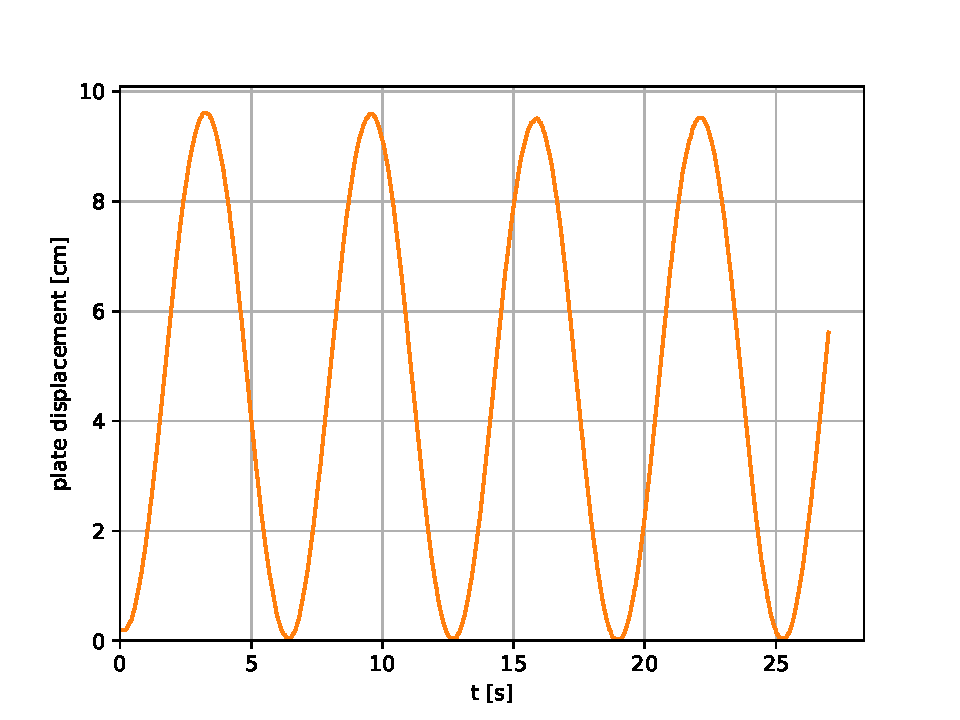
\includegraphics[width=0.45\textwidth, height=3.5cm]{graph/omega=0.50_A=5_plate.pdf}
&
\\
&
\\
&
\\
\end{tabular}
\end{center}
\begin{tikzpicture} [remember picture, overlay]
\node at (3.9, 8.7) {(a)};
\node at (10.8, 8.7) {(b)};
\node at (3.9, 5.0) {(c)};
\node at (10.8, 5.0) {(d)};
\node at (3.9, 1.4) {(e)};
\end{tikzpicture}
\caption{Plate movement - $\omega=3$ \\ (a) $A=1\mathrm{~cm}$ (b) $A=2\mathrm{~cm}$ (c) $A=3\mathrm{~cm}$ (d) $A=4\mathrm{~cm}$ (e) $A=5\mathrm{~cm}$\\(f) $A=6\mathrm{~cm}$ (g) $A=7\mathrm{~cm}$ (h) $A=8\mathrm{~cm}$ (i) $A=9\mathrm{~cm}$ (j) $A=10\mathrm{~cm}$}
\label{Data_omega=3_plate}
\end{figure}

\begin{figure}[H]
\begin{center}
\begin{tabular}{cc}
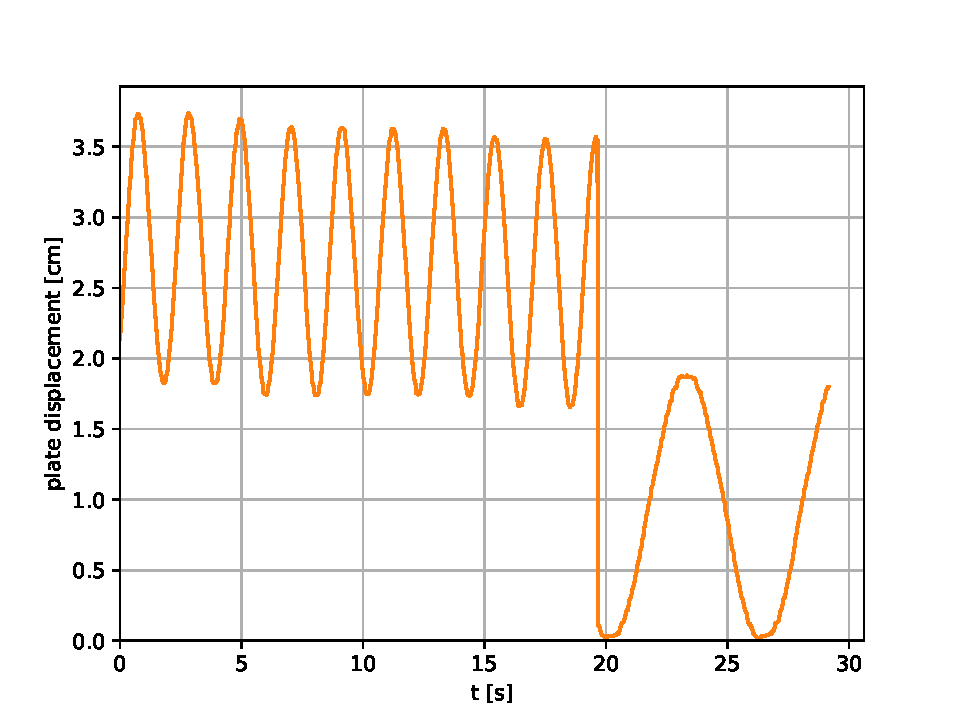
\includegraphics[width=0.45\textwidth, height=3.5cm]{graph/omega=1.00_A=1_plate.pdf}
&
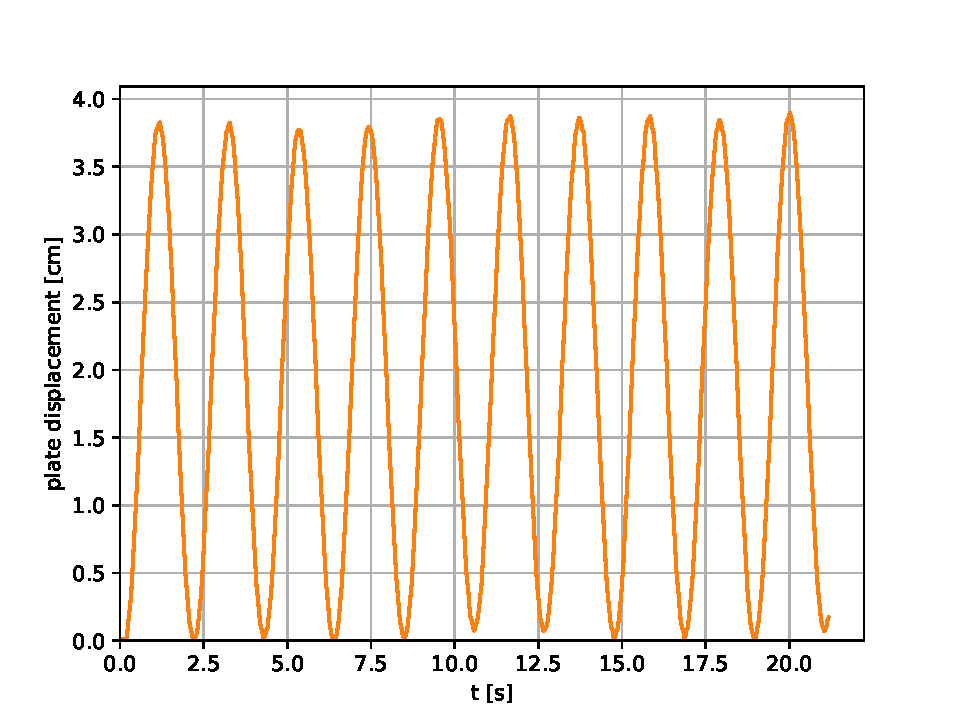
\includegraphics[width=0.45\textwidth, height=3.5cm]{graph/omega=1.00_A=2_plate.pdf}\\
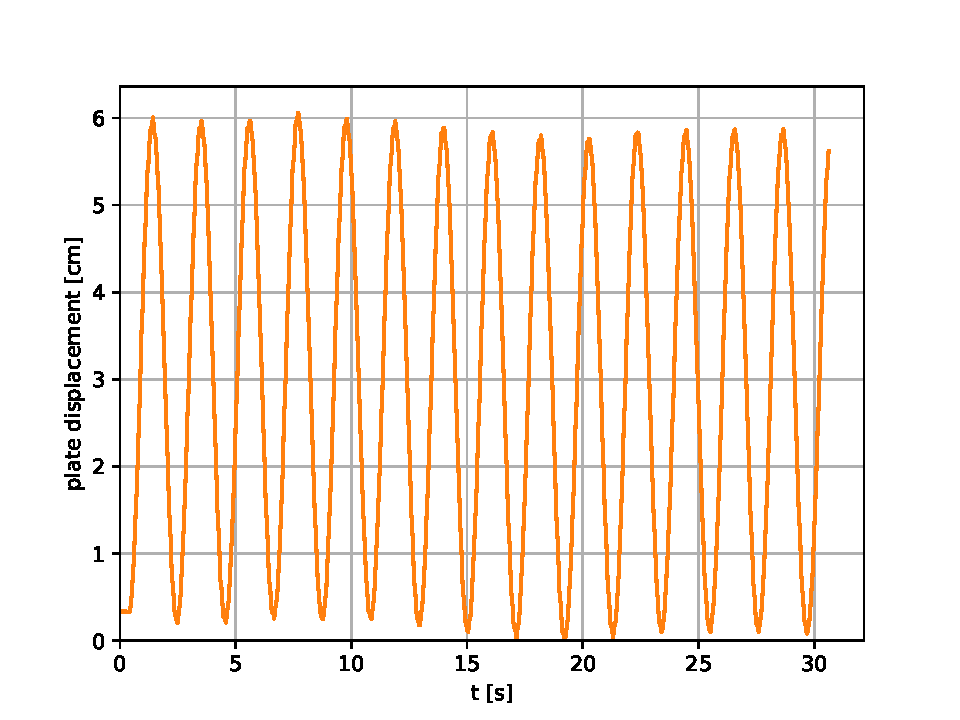
\includegraphics[width=0.45\textwidth, height=3.5cm]{graph/omega=1.00_A=3_plate.pdf}
&
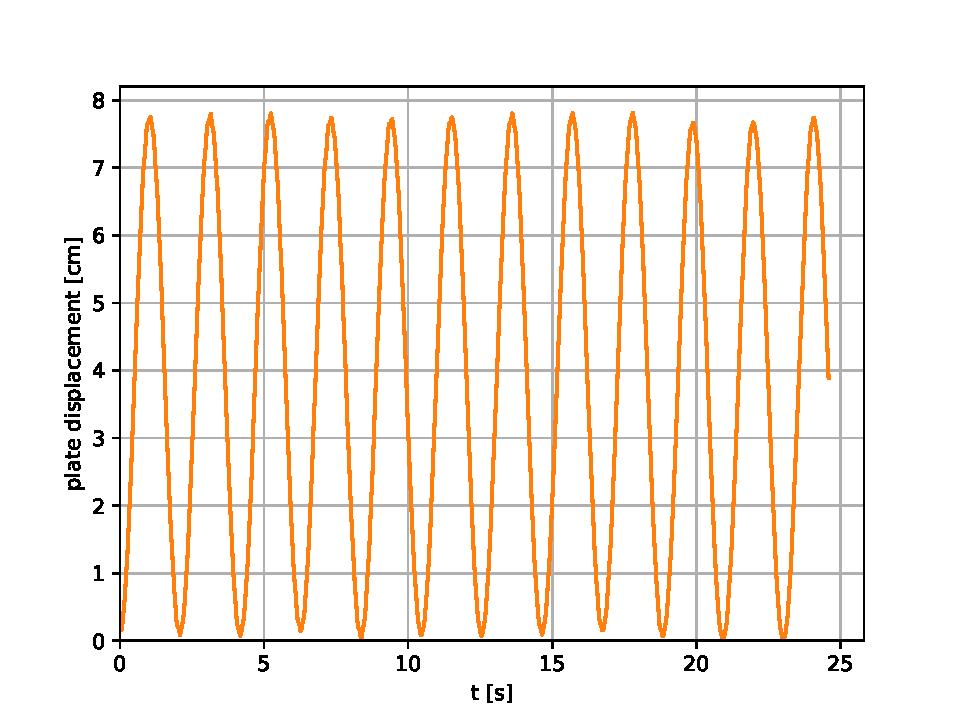
\includegraphics[width=0.45\textwidth, height=3.5cm]{graph/omega=1.00_A=4_plate.pdf}\\
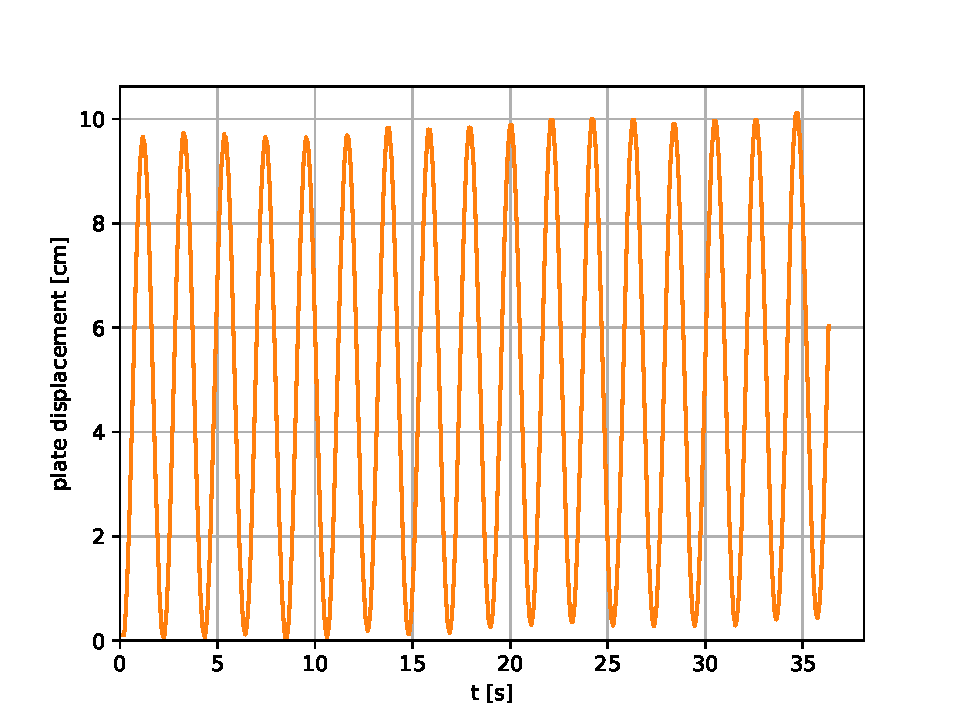
\includegraphics[width=0.45\textwidth, height=3.5cm]{graph/omega=1.00_A=5_plate.pdf}
&
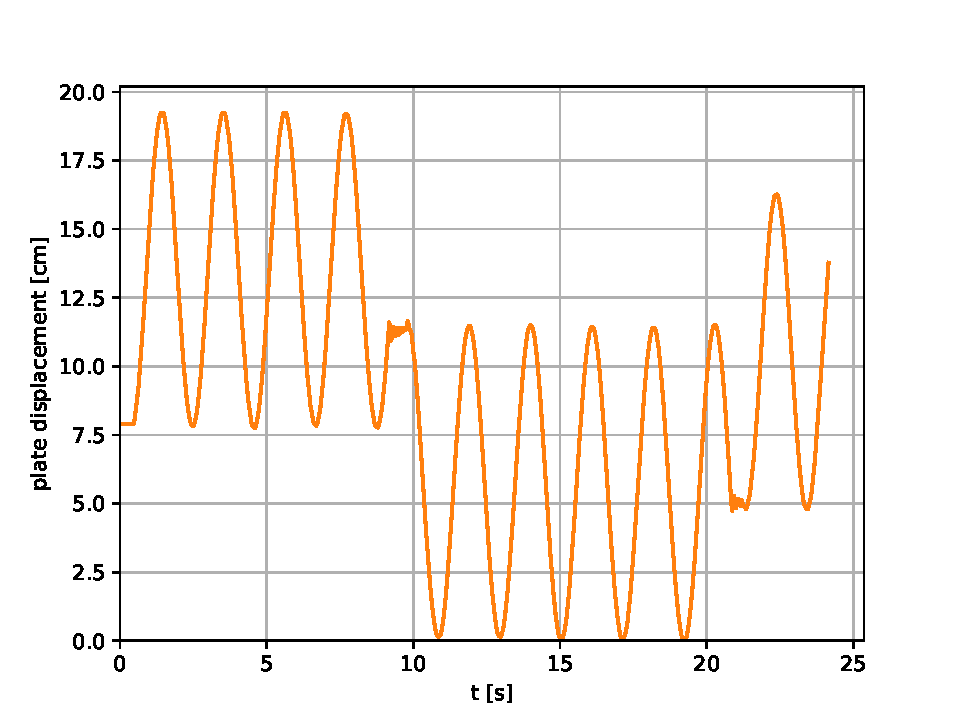
\includegraphics[width=0.45\textwidth, height=3.5cm]{graph/omega=1.00_A=6_plate.pdf}\\
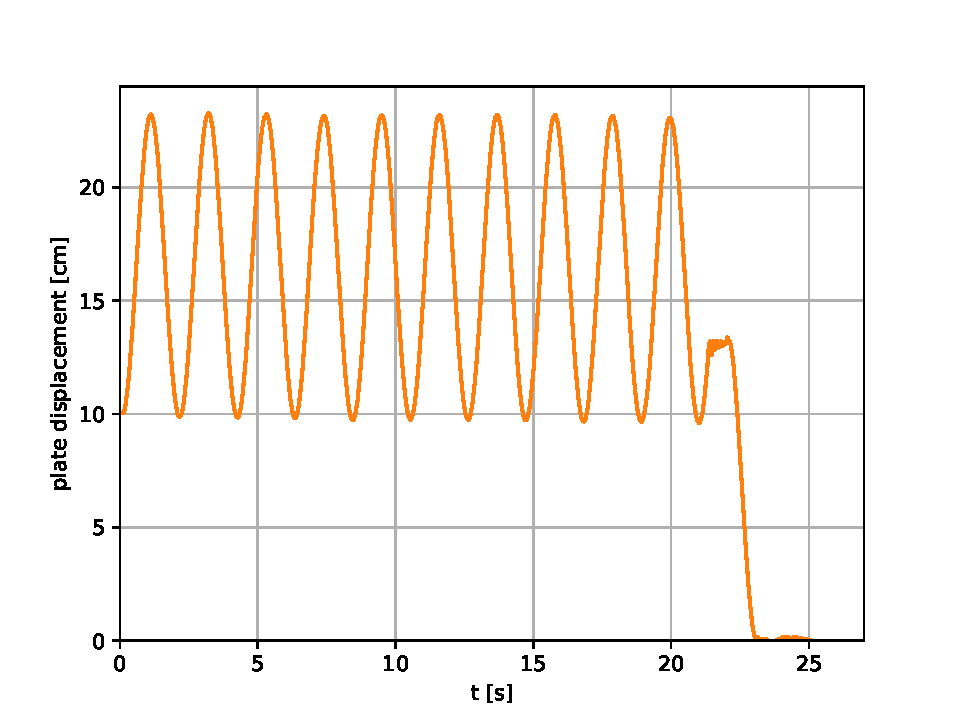
\includegraphics[width=0.45\textwidth, height=3.5cm]{graph/omega=1.00_A=7_plate.pdf}
&
\\
&
\\
\end{tabular}
\end{center}
\begin{tikzpicture} [remember picture, overlay]
\node at (3.9, 11.8) {(a)};
\node at (10.8, 11.8) {(b)};
\node at (3.9, 8.2) {(c)};
\node at (10.8, 8.2) {(d)};
\node at (3.9, 4.5) {(e)};
\node at (10.8, 4.5) {(f)};
\node at (3.9, 0.9) {(g)};
\end{tikzpicture}
\caption{Plate movement - $\omega=4$ \\ (a) $A=1\mathrm{~cm}$ (b) $A=2\mathrm{~cm}$ (c) $A=3\mathrm{~cm}$ (d) $A=4\mathrm{~cm}$ (e) $A=5\mathrm{~cm}$\\(f) $A=6\mathrm{~cm}$ (g) $A=7\mathrm{~cm}$ (h) $A=8\mathrm{~cm}$ (i) $A=9\mathrm{~cm}$ (j) $A=10\mathrm{~cm}$}
\label{Data_omega=4_plate}
\end{figure}

\begin{figure}[H]
\begin{center}
\begin{tabular}{cc}
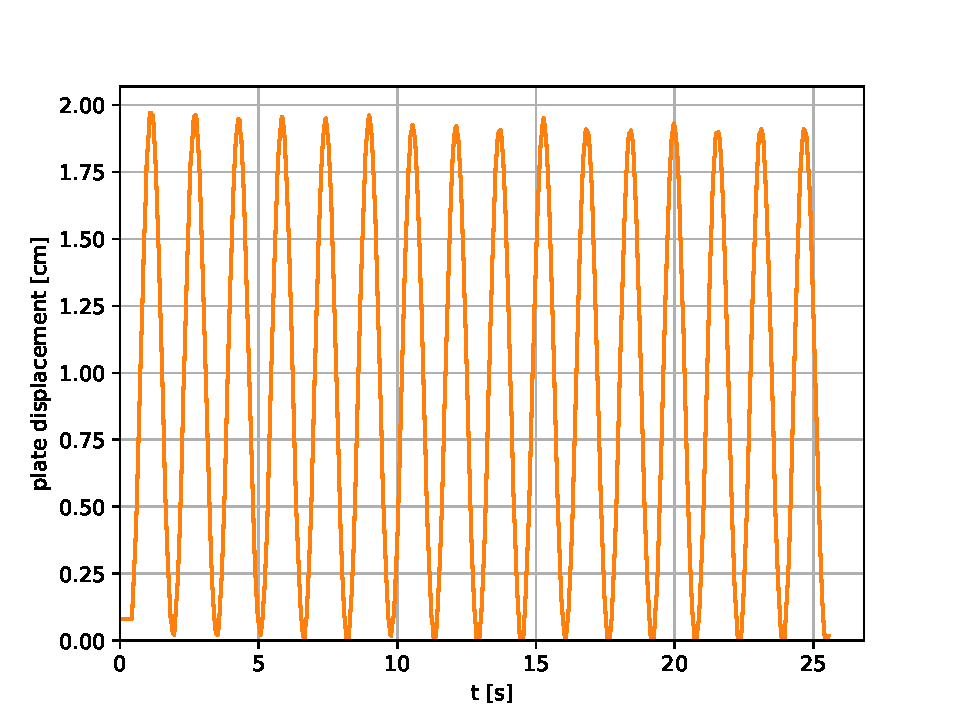
\includegraphics[width=0.45\textwidth, height=3.5cm]{graph/omega=1.50_A=1_plate.pdf}
&
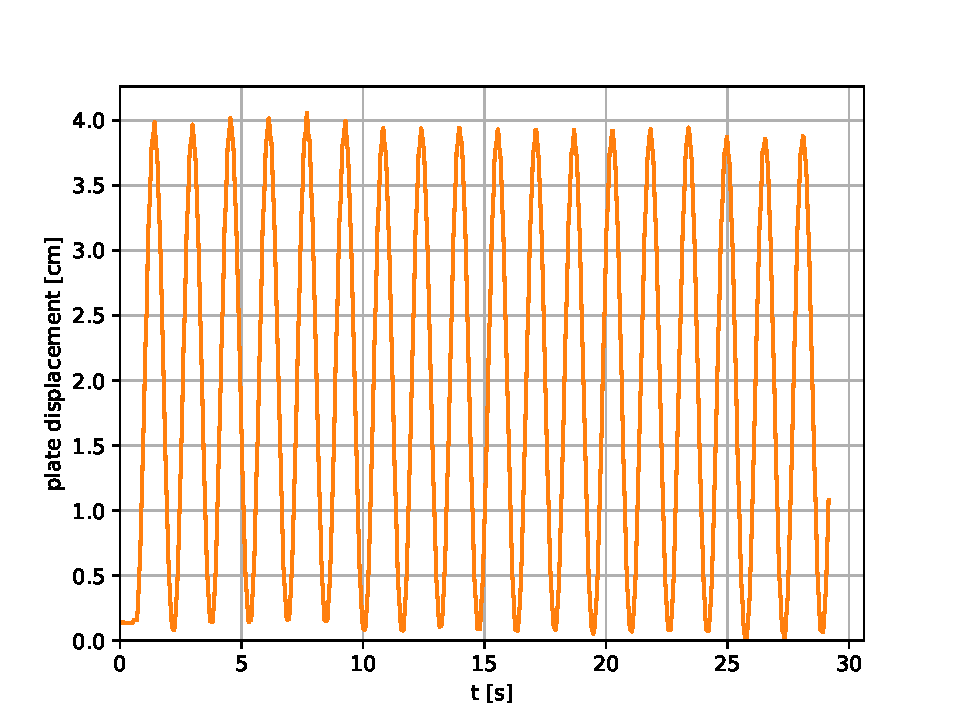
\includegraphics[width=0.45\textwidth, height=3.5cm]{graph/omega=1.50_A=2_plate.pdf}\\
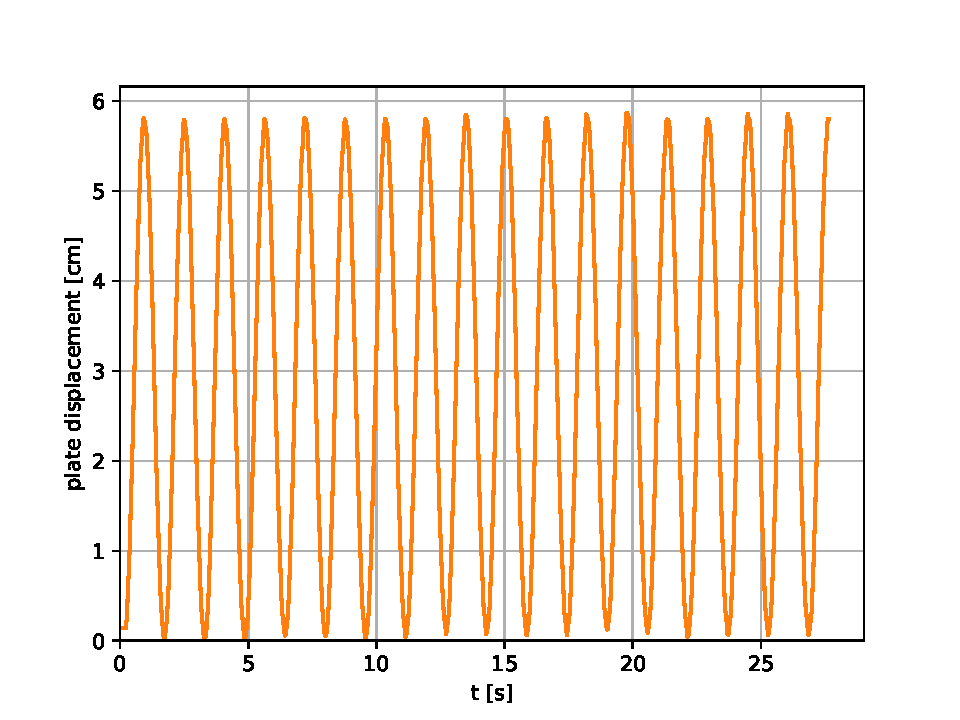
\includegraphics[width=0.45\textwidth, height=3.5cm]{graph/omega=1.50_A=3_plate.pdf}
&
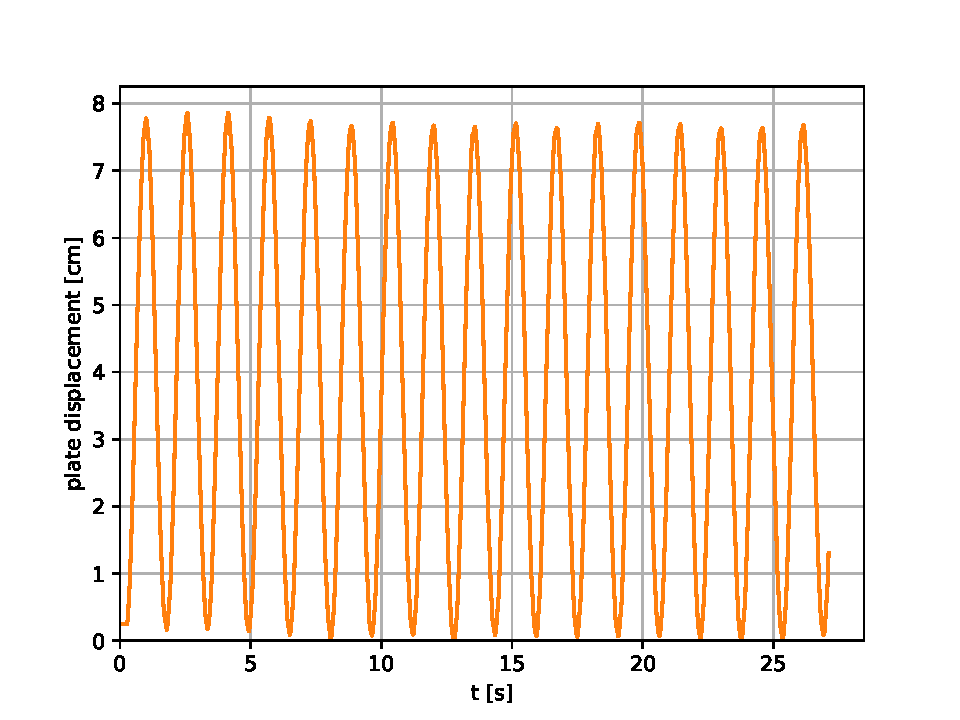
\includegraphics[width=0.45\textwidth, height=3.5cm]{graph/omega=1.50_A=4_plate.pdf}\\
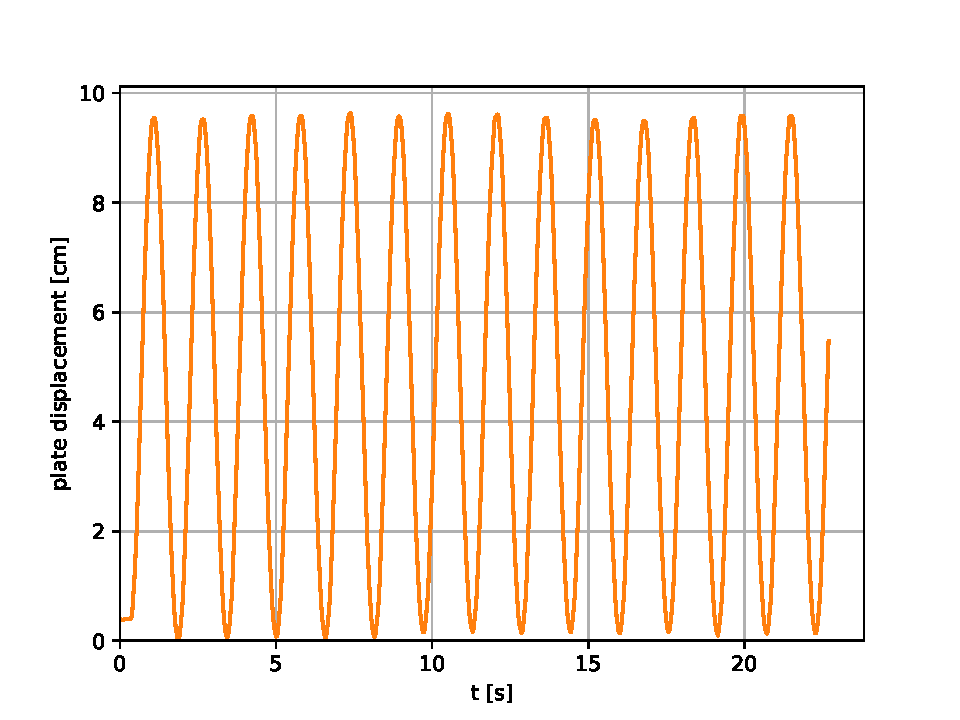
\includegraphics[width=0.45\textwidth, height=3.5cm]{graph/omega=1.50_A=5_plate.pdf}
&
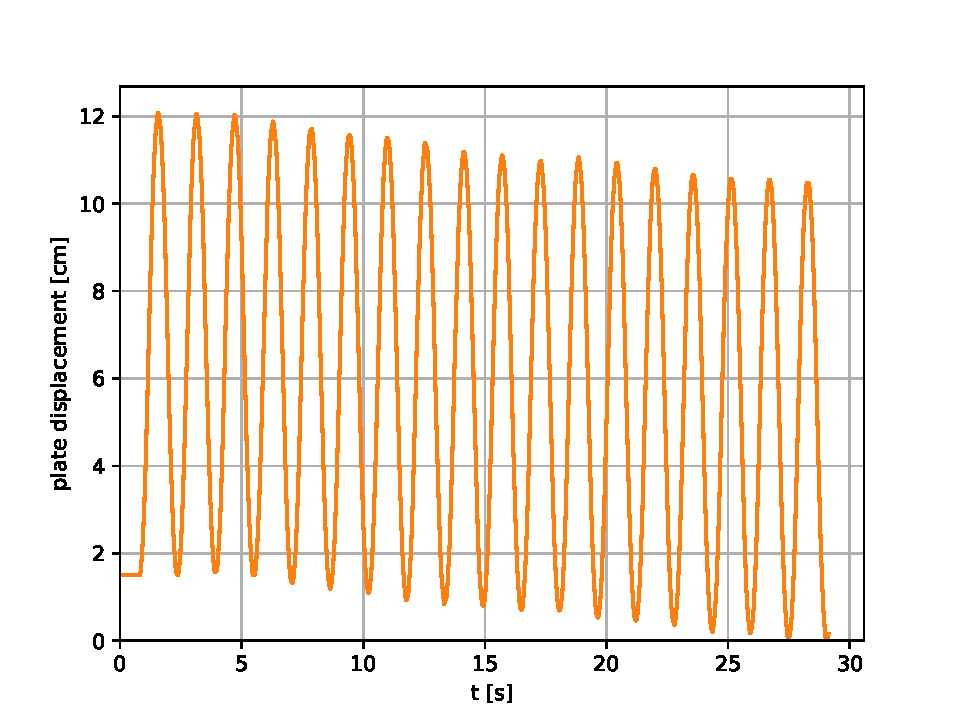
\includegraphics[width=0.45\textwidth, height=3.5cm]{graph/omega=1.50_A=6_plate.pdf}\\
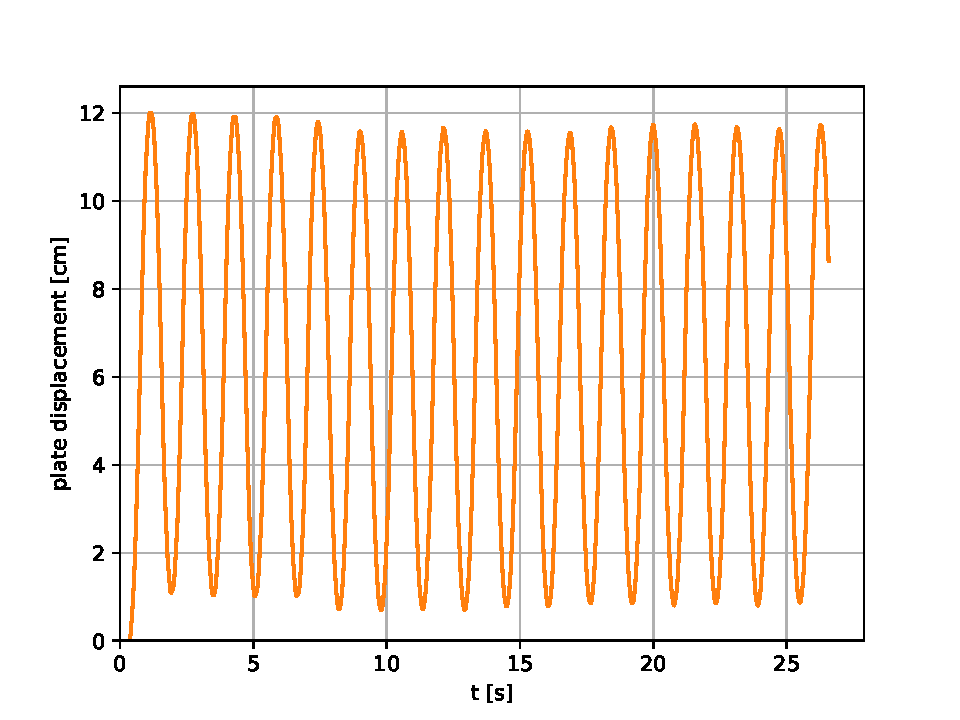
\includegraphics[width=0.45\textwidth, height=3.5cm]{graph/omega=1.50_A=7_plate.pdf}
&
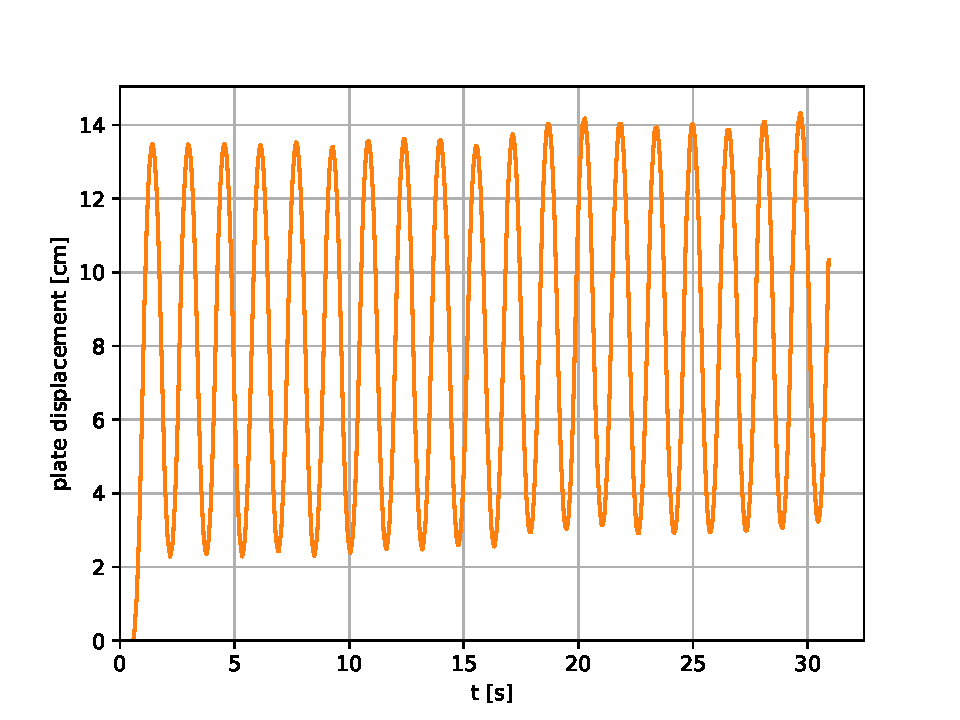
\includegraphics[width=0.45\textwidth, height=3.5cm]{graph/omega=1.50_A=8_plate.pdf}\\
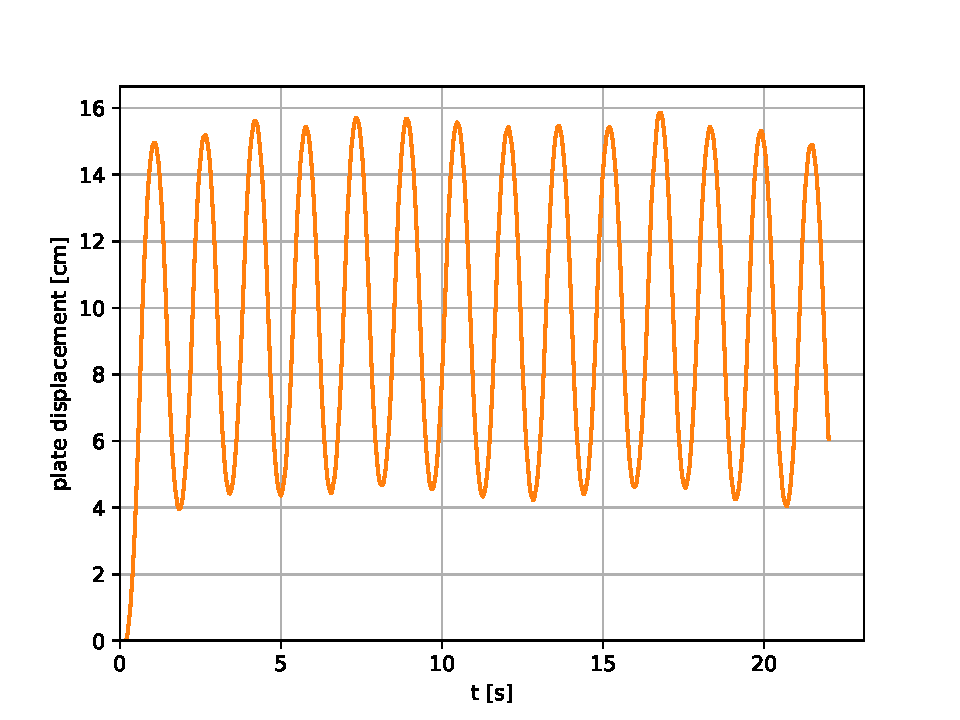
\includegraphics[width=0.45\textwidth, height=3.5cm]{graph/omega=1.50_A=9_plate.pdf}
&
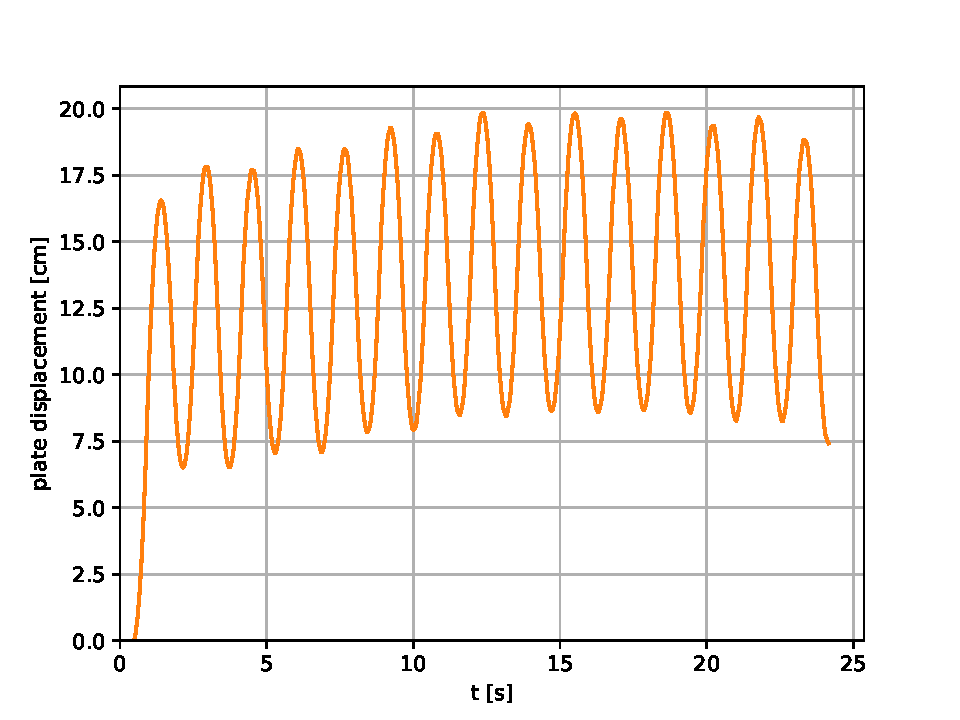
\includegraphics[width=0.45\textwidth, height=3.5cm]{graph/omega=1.50_A=10_plate.pdf}\\
\end{tabular}
\end{center}
\begin{tikzpicture} [remember picture, overlay]
\node at (3.9, 15.0) {(a)};
\node at (10.8, 15.0) {(b)};
\node at (3.9, 11.4) {(c)};
\node at (10.8, 11.4) {(d)};
\node at (3.9, 7.7) {(e)};
\node at (10.8, 7.7) {(f)};
\node at (3.9, 4.1) {(g)};
\node at (10.8, 4.1) {(h)};
\node at (3.9, 0.4) {(i)};
\node at (10.8, 0.4) {(j)};
\end{tikzpicture}
\caption{Plate movement - $\omega=6$ \\ (a) $A=1\mathrm{~cm}$ (b) $A=2\mathrm{~cm}$ (c) $A=3\mathrm{~cm}$ (d) $A=4\mathrm{~cm}$ (e) $A=5\mathrm{~cm}$\\(f) $A=6\mathrm{~cm}$ (g) $A=7\mathrm{~cm}$ (h) $A=8\mathrm{~cm}$ (i) $A=9\mathrm{~cm}$ (j) $A=10\mathrm{~cm}$}
\label{Data_omega=6_plate}
\end{figure}

\begin{figure}[H]
\begin{center}
\begin{tabular}{cc}
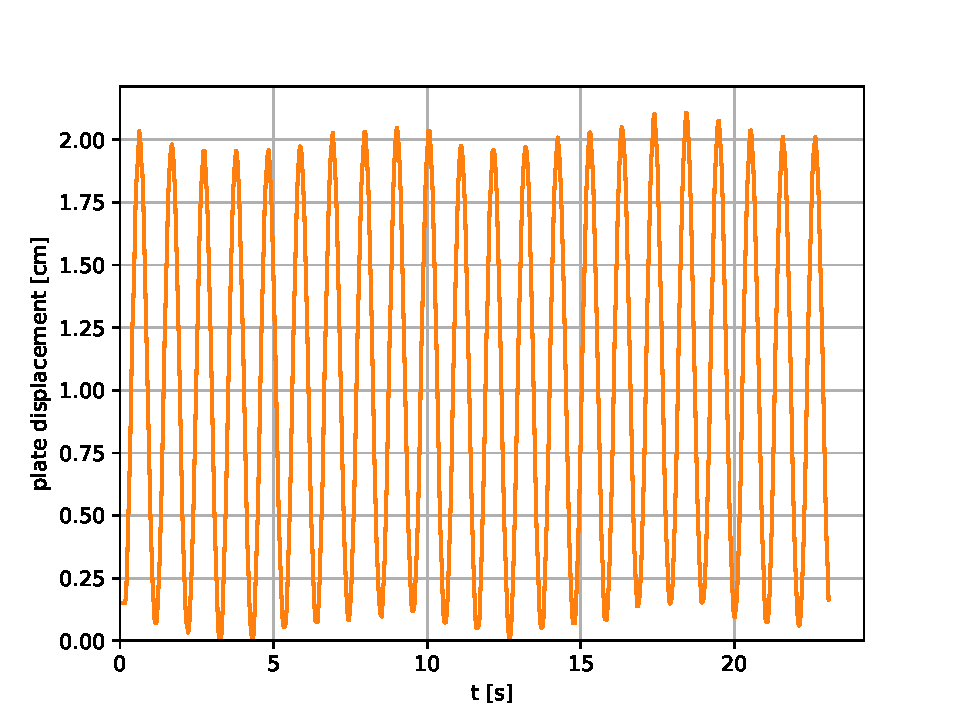
\includegraphics[width=0.45\textwidth, height=3.5cm]{graph/omega=2.00_A=1_plate.pdf}
&
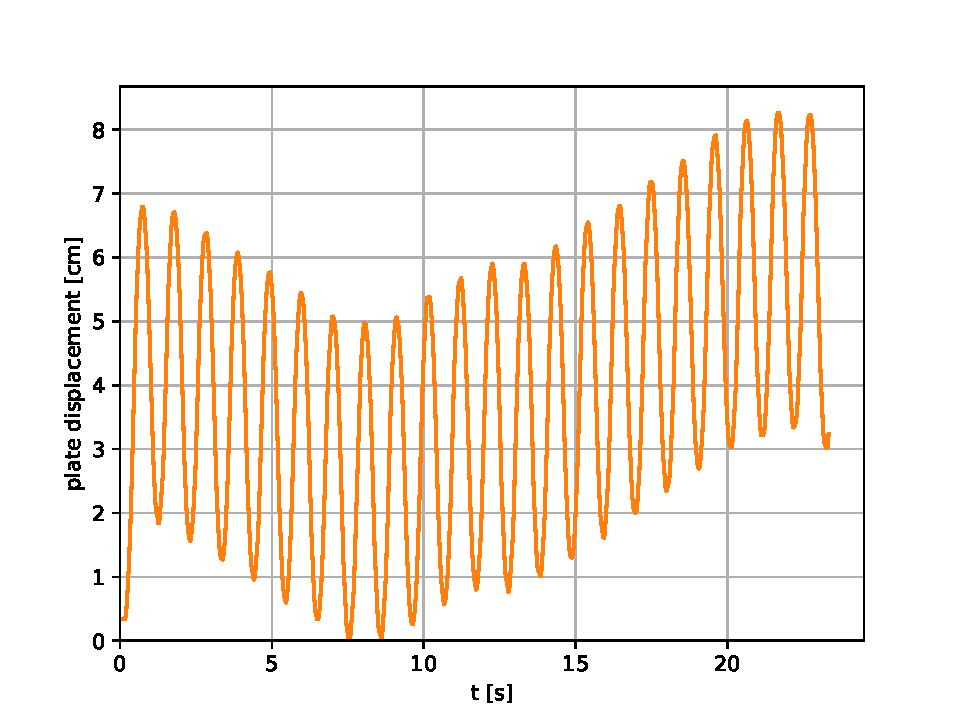
\includegraphics[width=0.45\textwidth, height=3.5cm]{graph/omega=2.00_A=2_plate.pdf}\\
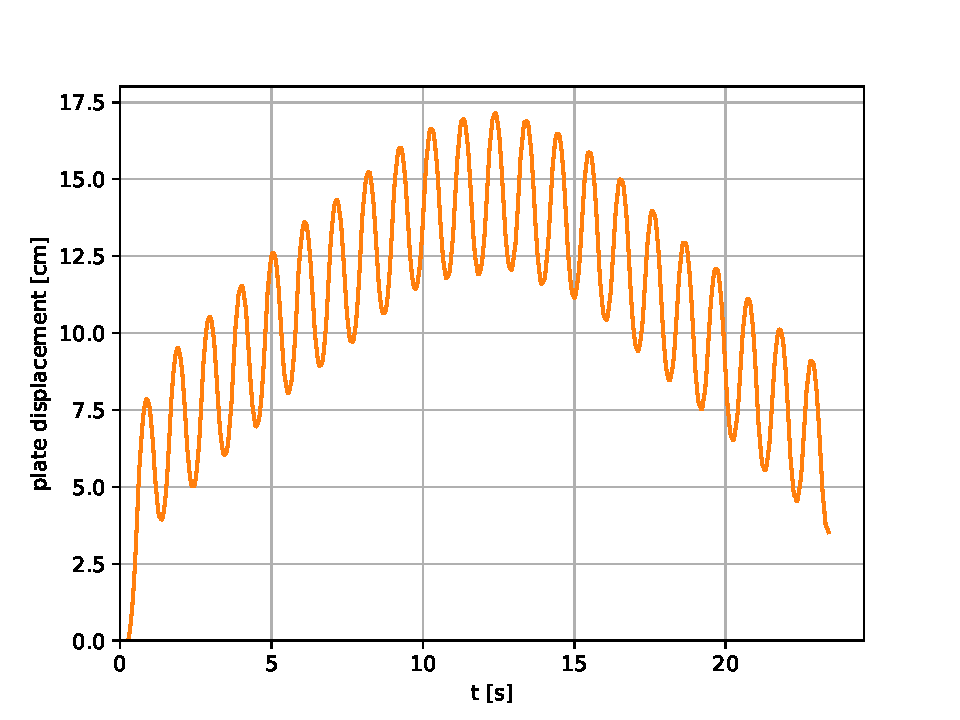
\includegraphics[width=0.45\textwidth, height=3.5cm]{graph/omega=2.00_A=3_plate.pdf}
&
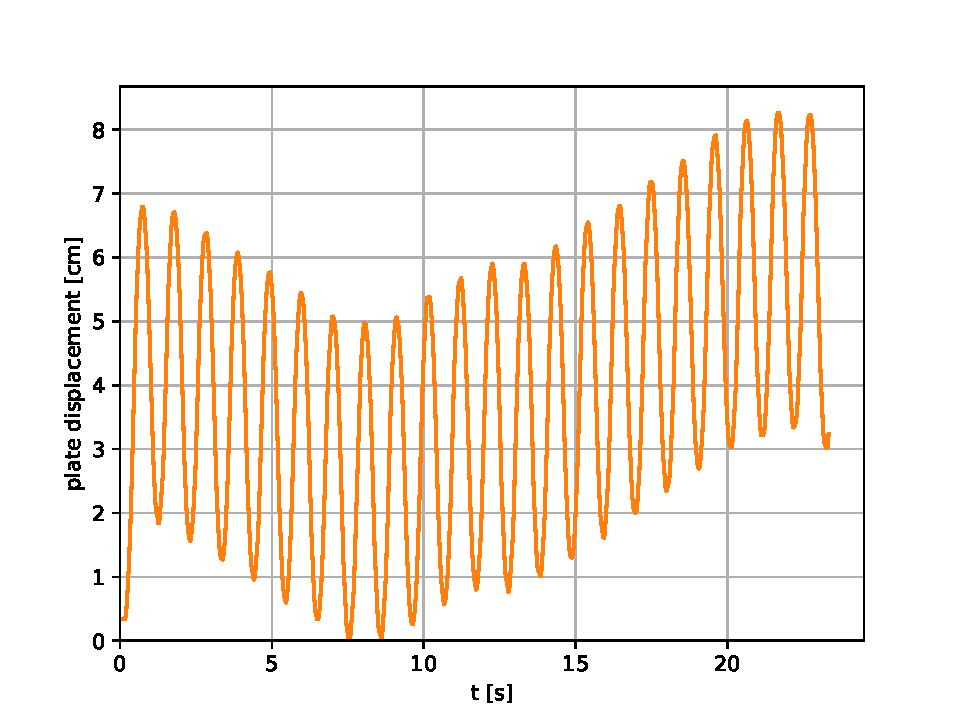
\includegraphics[width=0.45\textwidth, height=3.5cm]{graph/omega=2.00_A=4_plate.pdf}\\
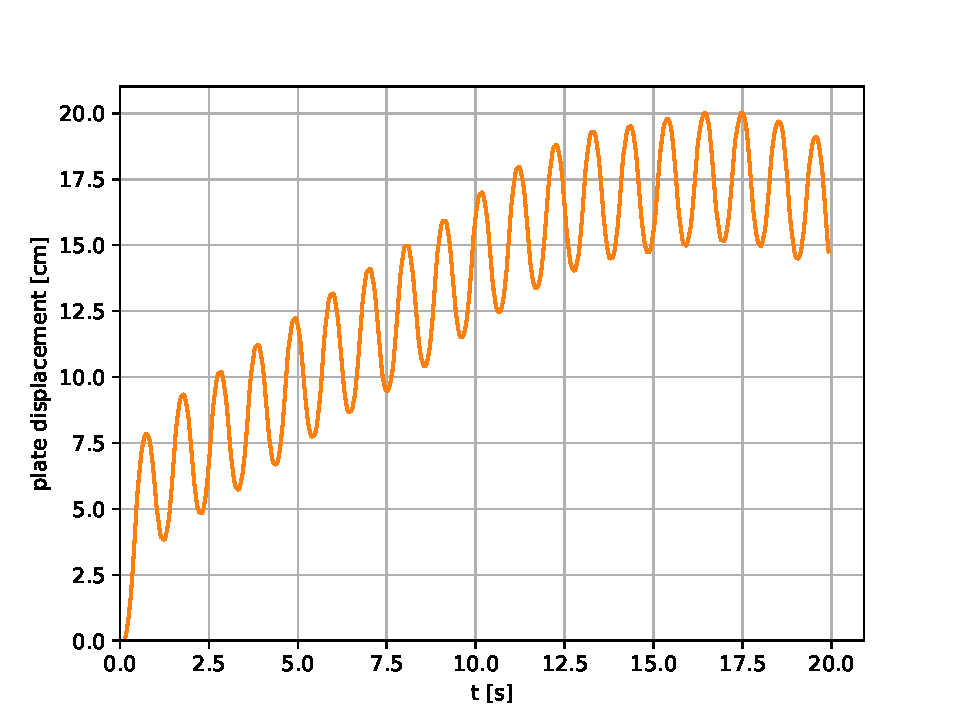
\includegraphics[width=0.45\textwidth, height=3.5cm]{graph/omega=2.00_A=5_plate.pdf}
&
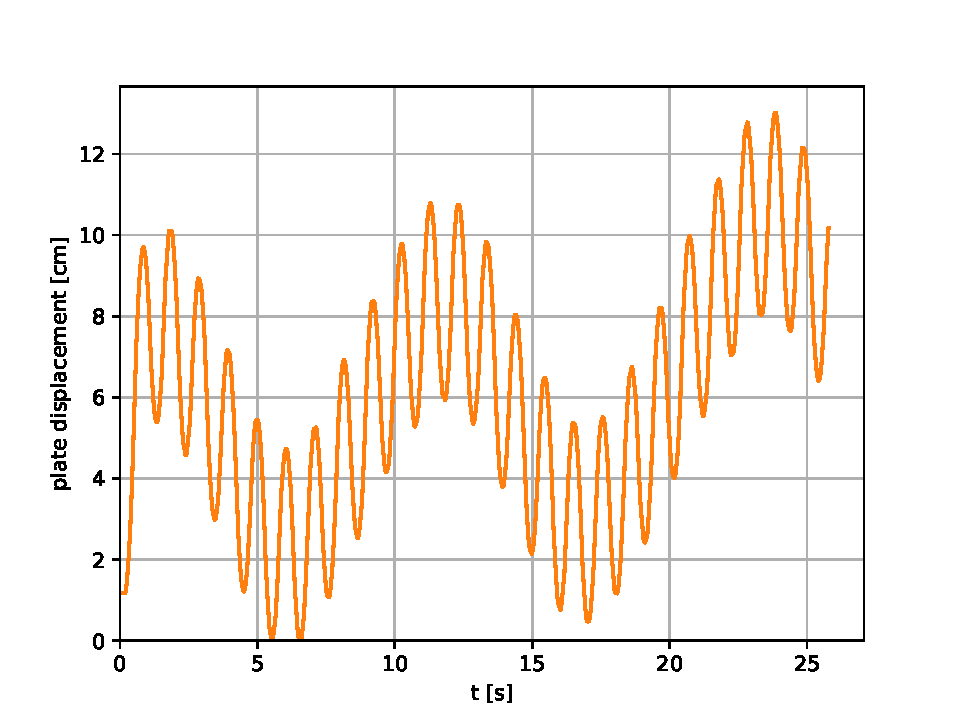
\includegraphics[width=0.45\textwidth, height=3.5cm]{graph/omega=2.00_A=6_plate.pdf}\\
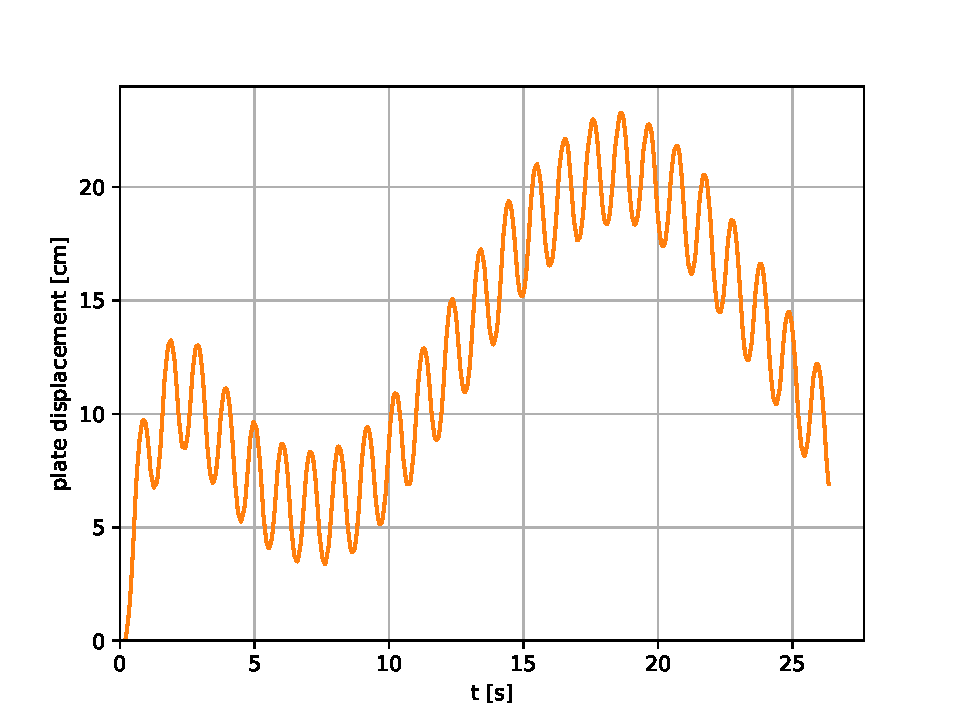
\includegraphics[width=0.45\textwidth, height=3.5cm]{graph/omega=2.00_A=7_plate.pdf}
&
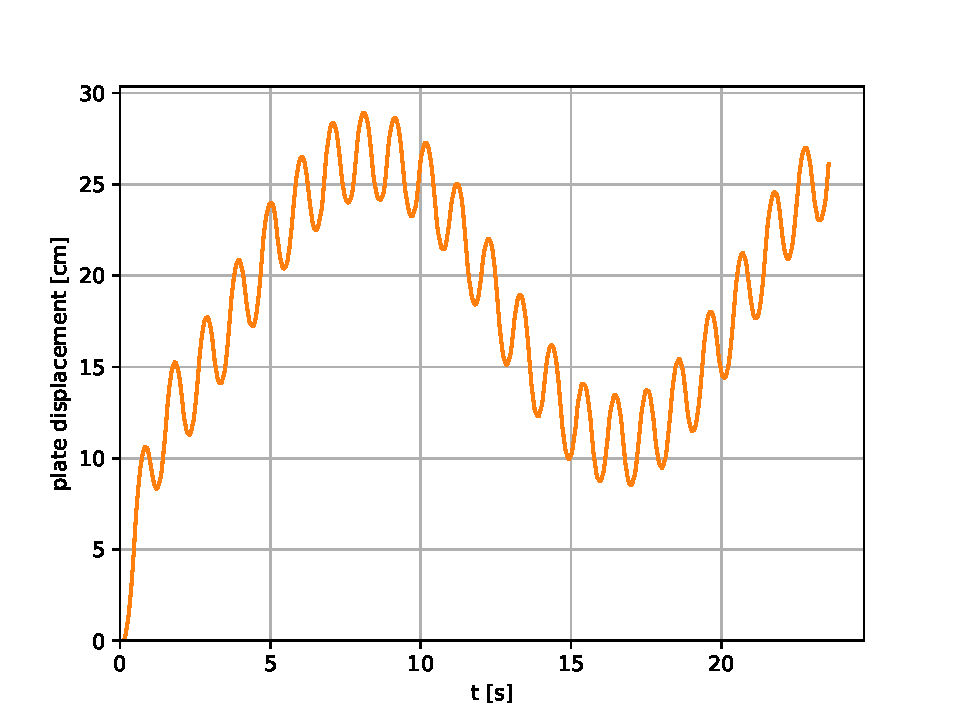
\includegraphics[width=0.45\textwidth, height=3.5cm]{graph/omega=2.00_A=8_plate.pdf}\\
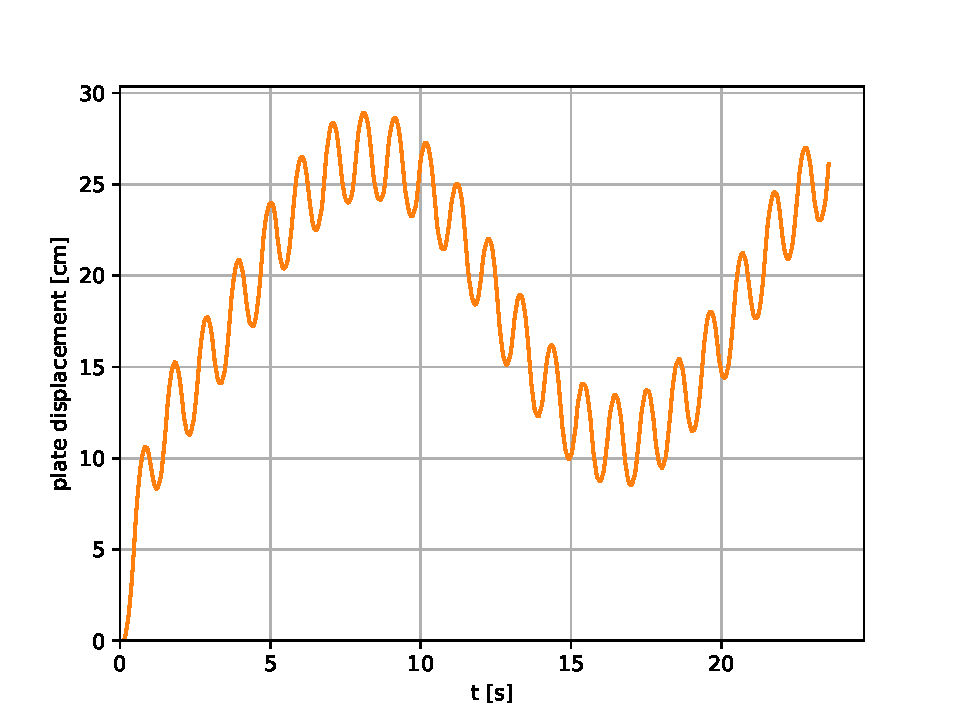
\includegraphics[width=0.45\textwidth, height=3.5cm]{graph/omega=2.00_A=9_plate.pdf}
&
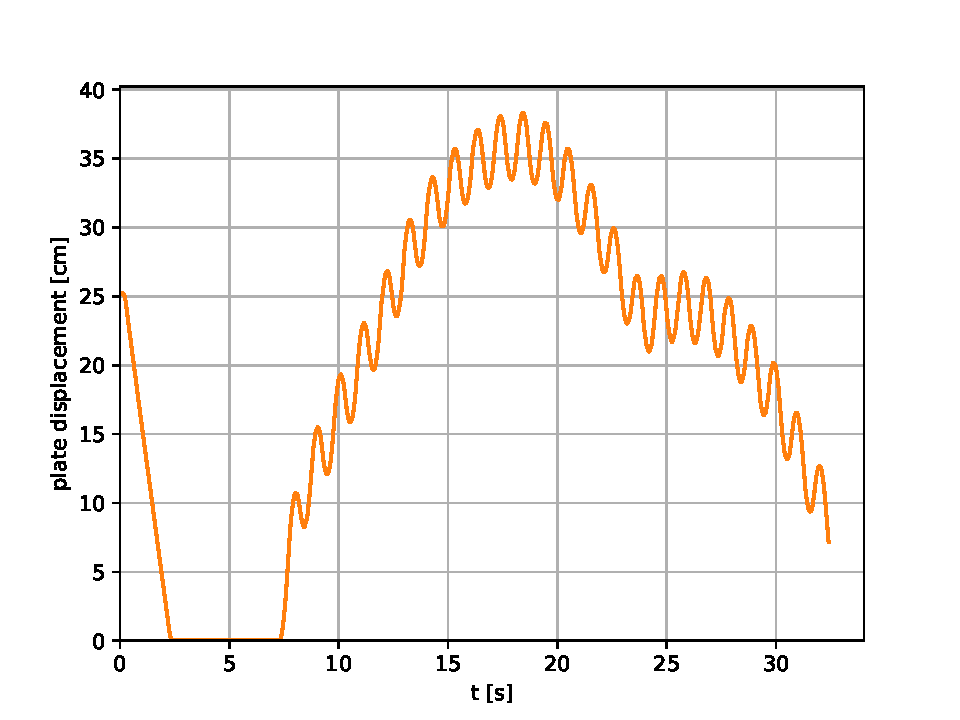
\includegraphics[width=0.45\textwidth, height=3.5cm]{graph/omega=2.00_A=10_plate.pdf}\\
\end{tabular}
\end{center}
\begin{tikzpicture} [remember picture, overlay]
\node at (3.9, 15.0) {(a)};
\node at (10.8, 15.0) {(b)};
\node at (3.9, 11.4) {(c)};
\node at (10.8, 11.4) {(d)};
\node at (3.9, 7.7) {(e)};
\node at (10.8, 7.7) {(f)};
\node at (3.9, 4.1) {(g)};
\node at (10.8, 4.1) {(h)};
\node at (3.9, 0.4) {(i)};
\node at (10.8, 0.4) {(j)};
\end{tikzpicture}
\caption{Plate movement - $\omega=7$ \\ (a) $A=1\mathrm{~cm}$ (b) $A=2\mathrm{~cm}$ (c) $A=3\mathrm{~cm}$ (d) $A=4\mathrm{~cm}$ (e) $A=5\mathrm{~cm}$\\(f) $A=6\mathrm{~cm}$ (g) $A=7\mathrm{~cm}$ (h) $A=8\mathrm{~cm}$ (i) $A=9\mathrm{~cm}$ (j) $A=10\mathrm{~cm}$}
\label{Data_omega=7_plate}
\end{figure}

\begin{figure}[H]
\begin{center}
\begin{tabular}{cc}
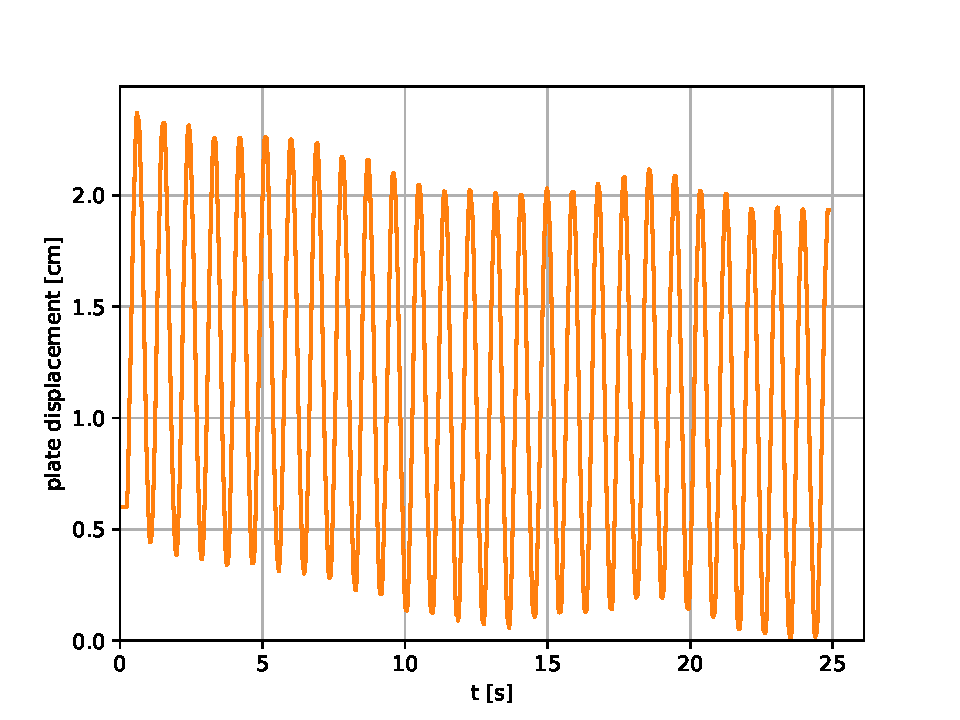
\includegraphics[width=0.45\textwidth, height=3.5cm]{graph/omega=2.50_A=1_plate.pdf}
&
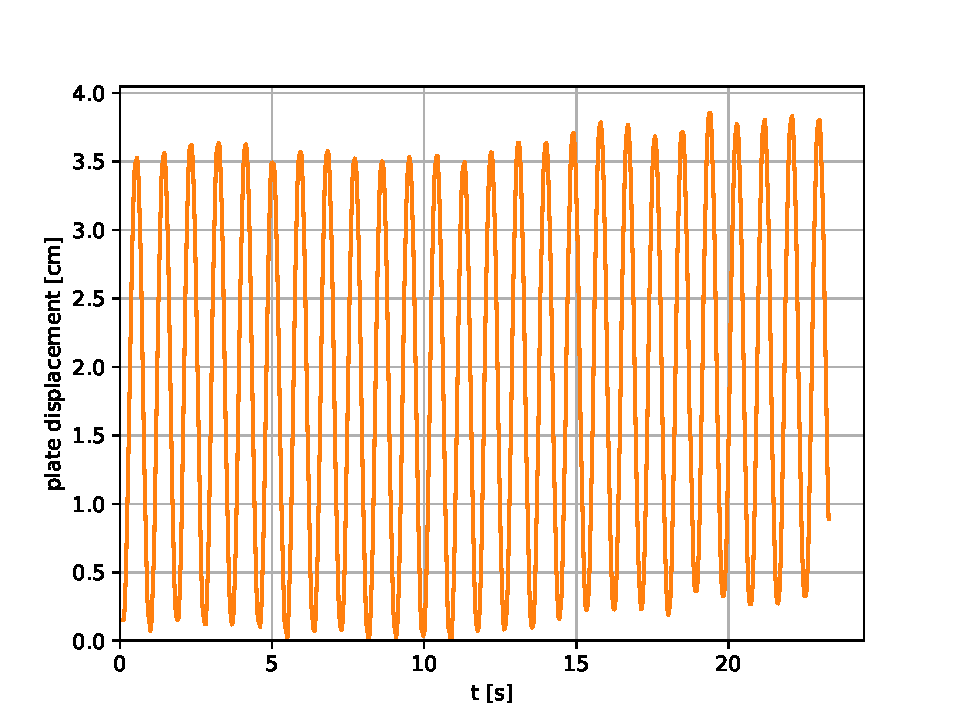
\includegraphics[width=0.45\textwidth, height=3.5cm]{graph/omega=2.50_A=2_plate.pdf}\\
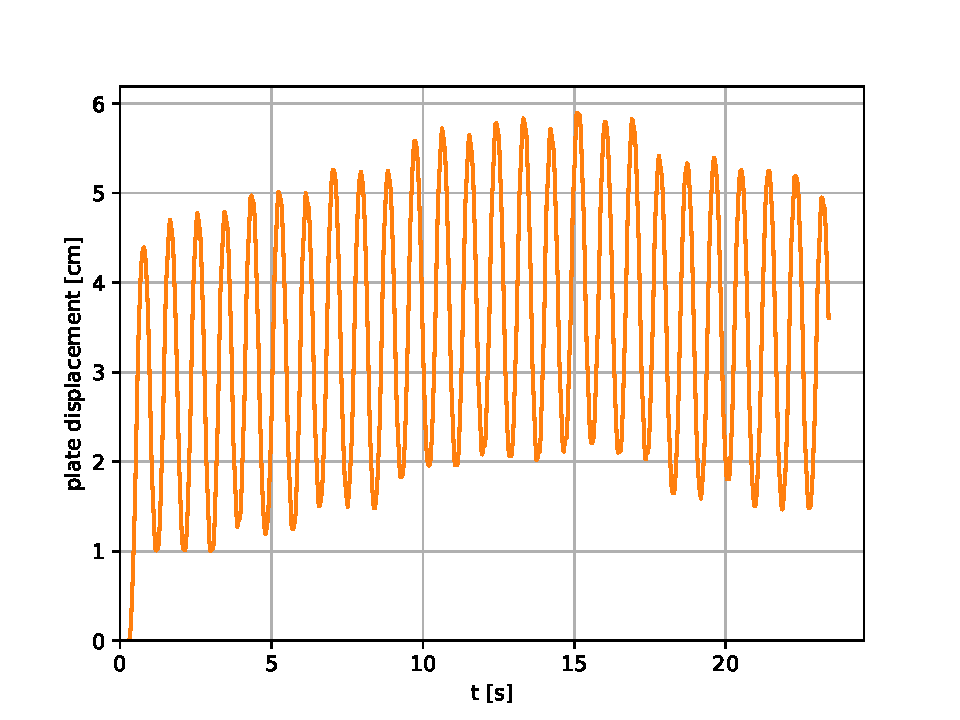
\includegraphics[width=0.45\textwidth, height=3.5cm]{graph/omega=2.50_A=3_plate.pdf}
&
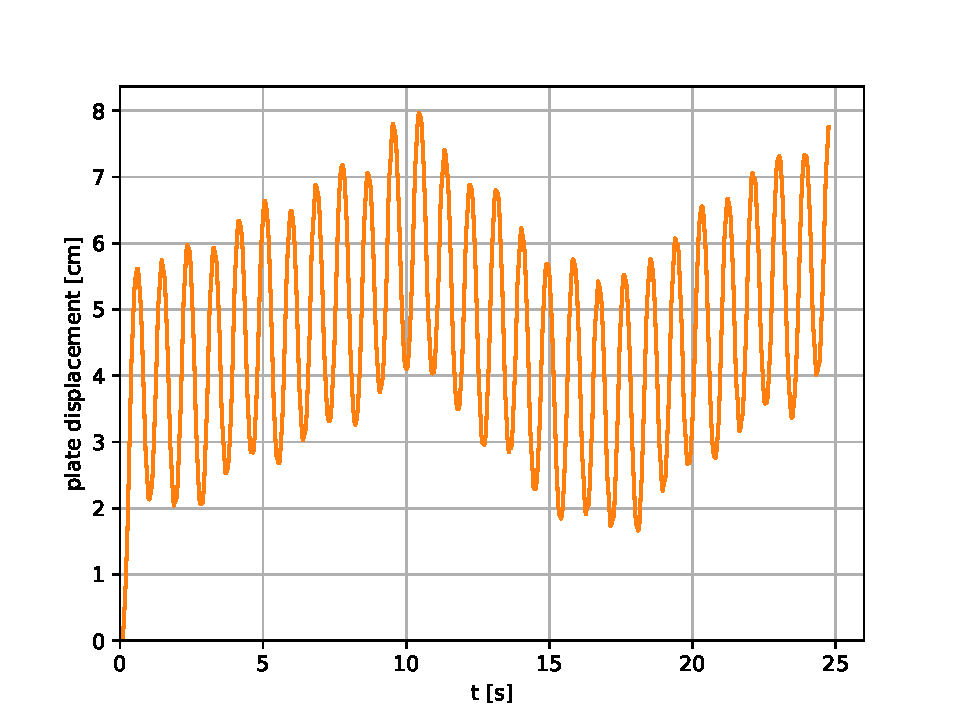
\includegraphics[width=0.45\textwidth, height=3.5cm]{graph/omega=2.50_A=4_plate.pdf}\\
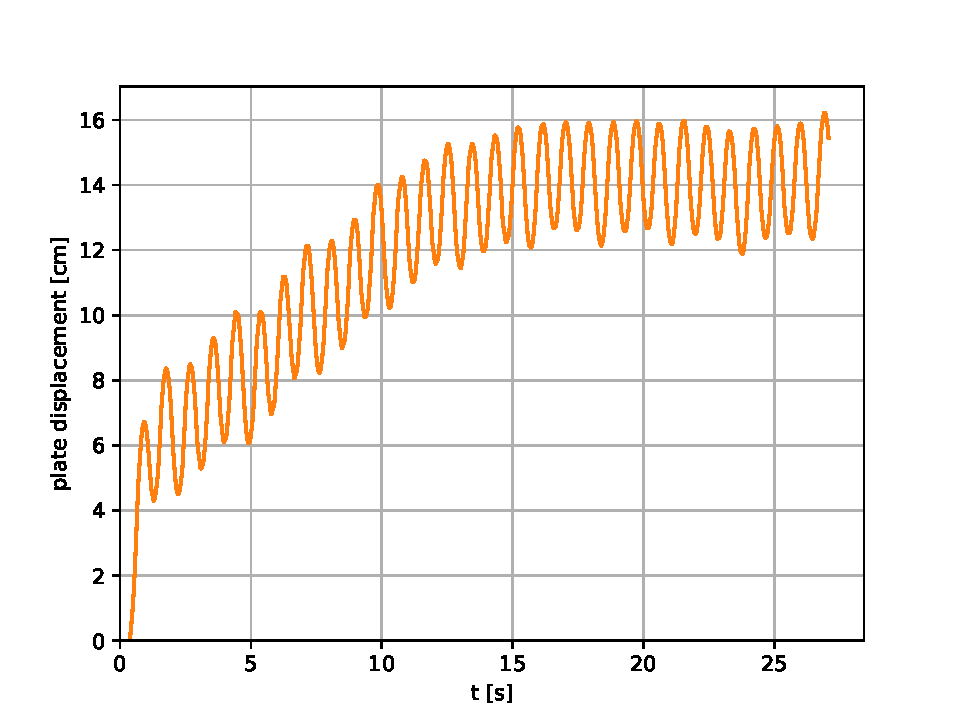
\includegraphics[width=0.45\textwidth, height=3.5cm]{graph/omega=2.50_A=5_plate.pdf}
&
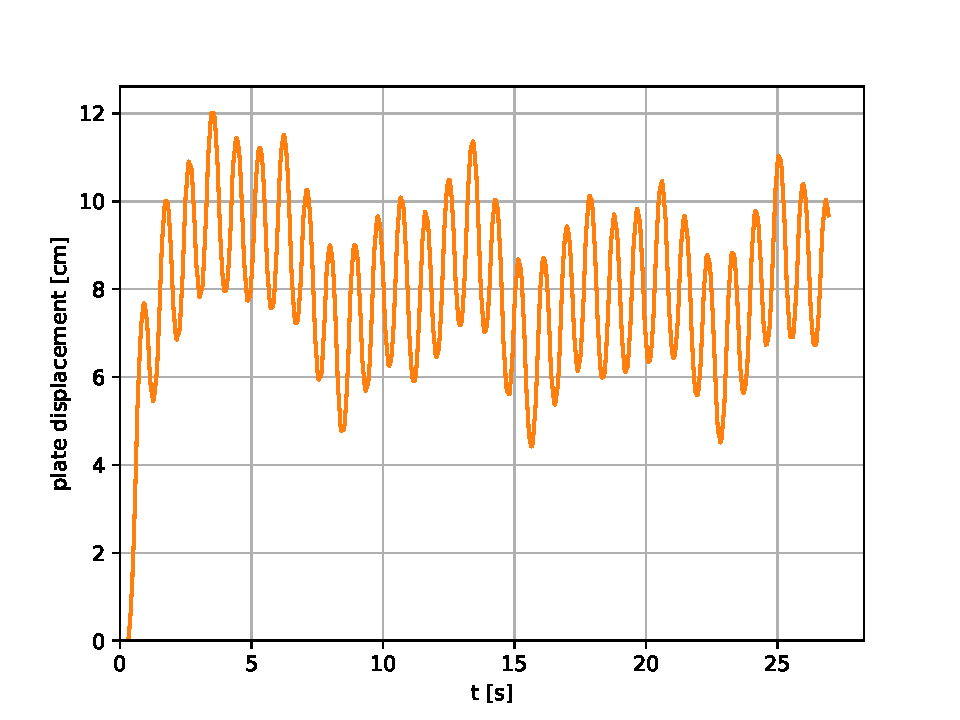
\includegraphics[width=0.45\textwidth, height=3.5cm]{graph/omega=2.50_A=6_plate.pdf}\\
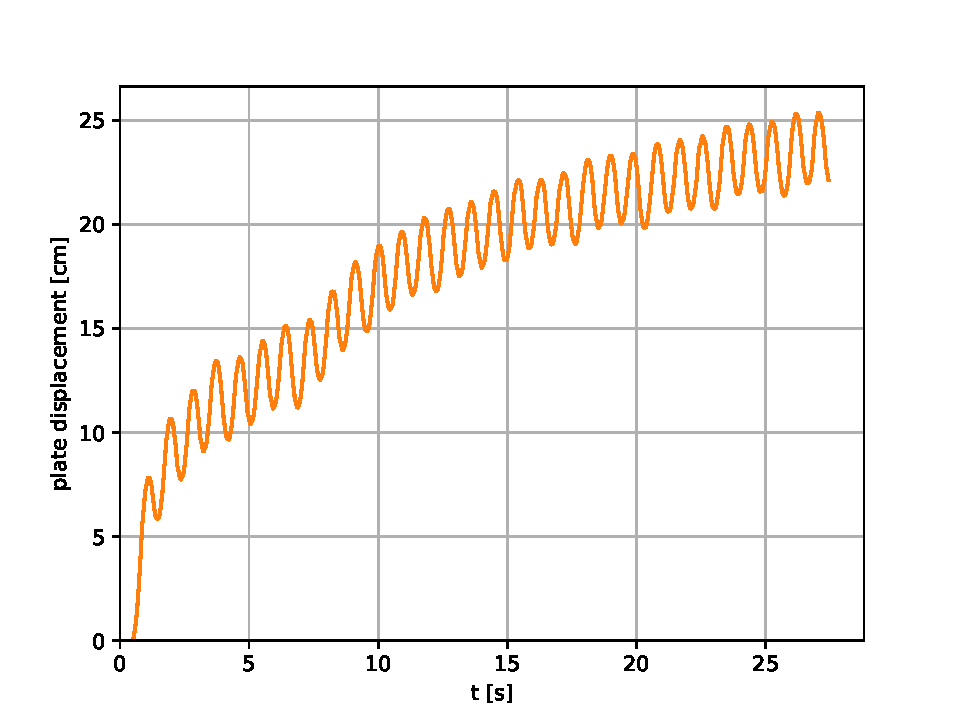
\includegraphics[width=0.45\textwidth, height=3.5cm]{graph/omega=2.50_A=7_plate.pdf}
&
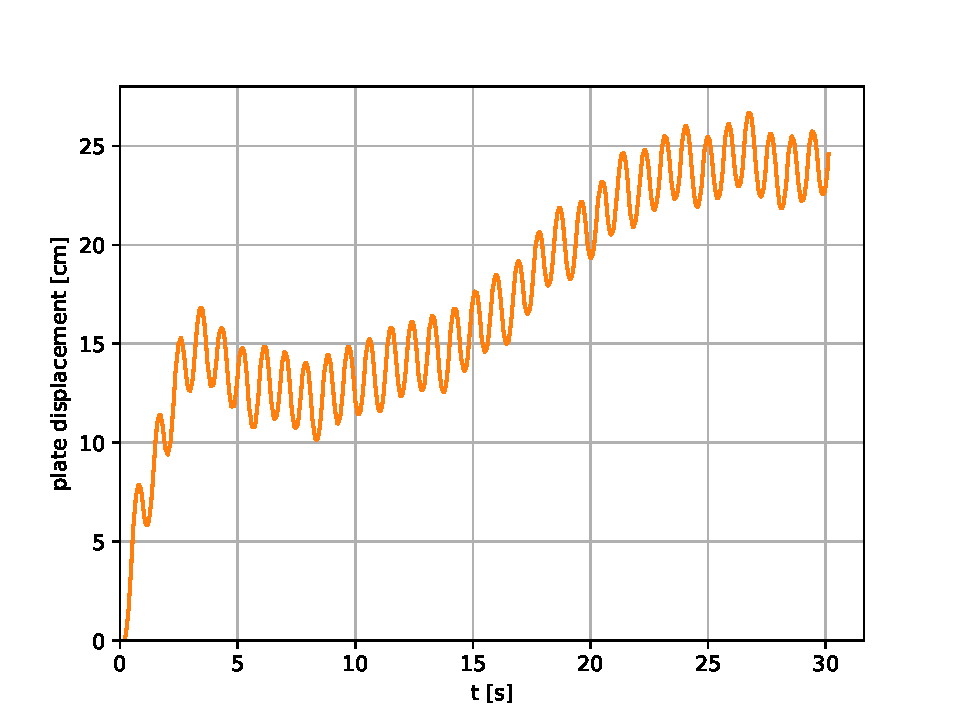
\includegraphics[width=0.45\textwidth, height=3.5cm]{graph/omega=2.50_A=8_plate.pdf}\\
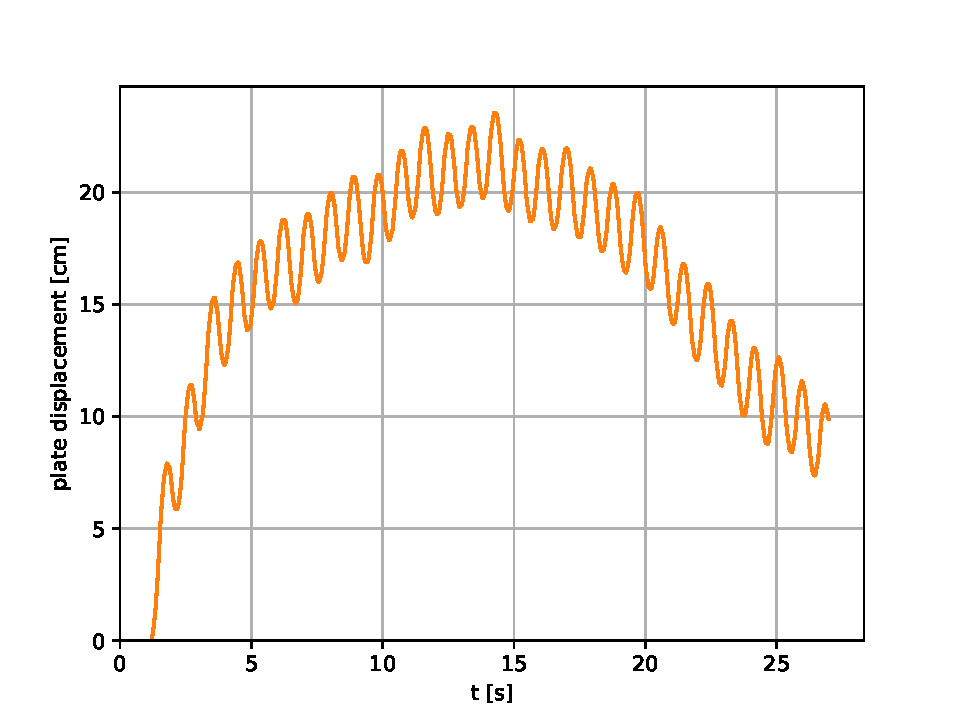
\includegraphics[width=0.45\textwidth, height=3.5cm]{graph/omega=2.50_A=9_plate.pdf}
&
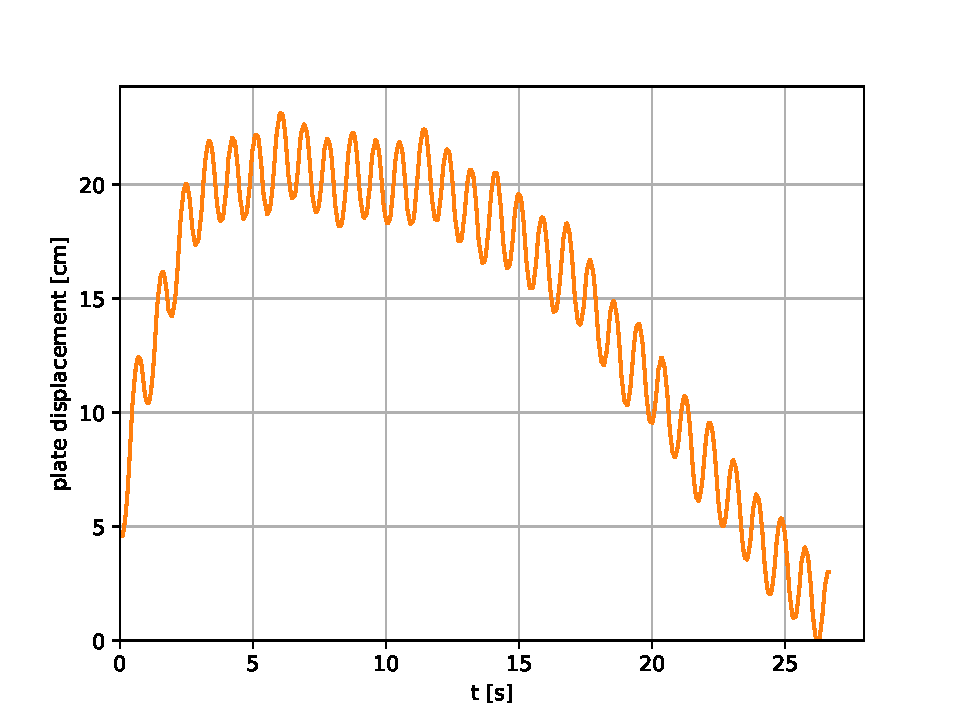
\includegraphics[width=0.45\textwidth, height=3.5cm]{graph/omega=2.50_A=10_plate.pdf}\\
\end{tabular}
\end{center}
\begin{tikzpicture} [remember picture, overlay]
\node at (3.9, 15.0) {(a)};
\node at (10.8, 15.0) {(b)};
\node at (3.9, 11.4) {(c)};
\node at (10.8, 11.4) {(d)};
\node at (3.9, 7.7) {(e)};
\node at (10.8, 7.7) {(f)};
\node at (3.9, 4.1) {(g)};
\node at (10.8, 4.1) {(h)};
\node at (3.9, 0.4) {(i)};
\node at (10.8, 0.4) {(j)};
\end{tikzpicture}
\caption{Plate movement - $\omega=9$ \\ (a) $A=1\mathrm{~cm}$ (b) $A=2\mathrm{~cm}$ (c) $A=3\mathrm{~cm}$ (d) $A=4\mathrm{~cm}$ (e) $A=5\mathrm{~cm}$\\(f) $A=6\mathrm{~cm}$ (g) $A=7\mathrm{~cm}$ (h) $A=8\mathrm{~cm}$ (i) $A=9\mathrm{~cm}$ (j) $A=10\mathrm{~cm}$}
\label{Data_omega=9_plate}
\end{figure}

\begin{figure}[H]
\begin{center}
\begin{tabular}{cc}
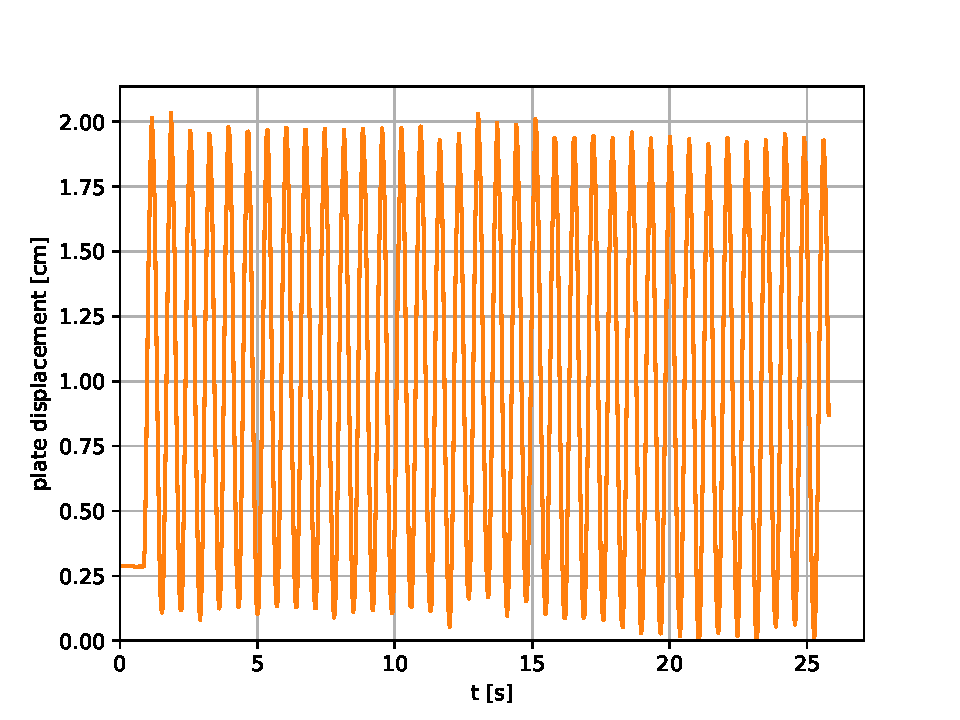
\includegraphics[width=0.45\textwidth, height=3.5cm]{graph/omega=3.00_A=1_plate.pdf}
&
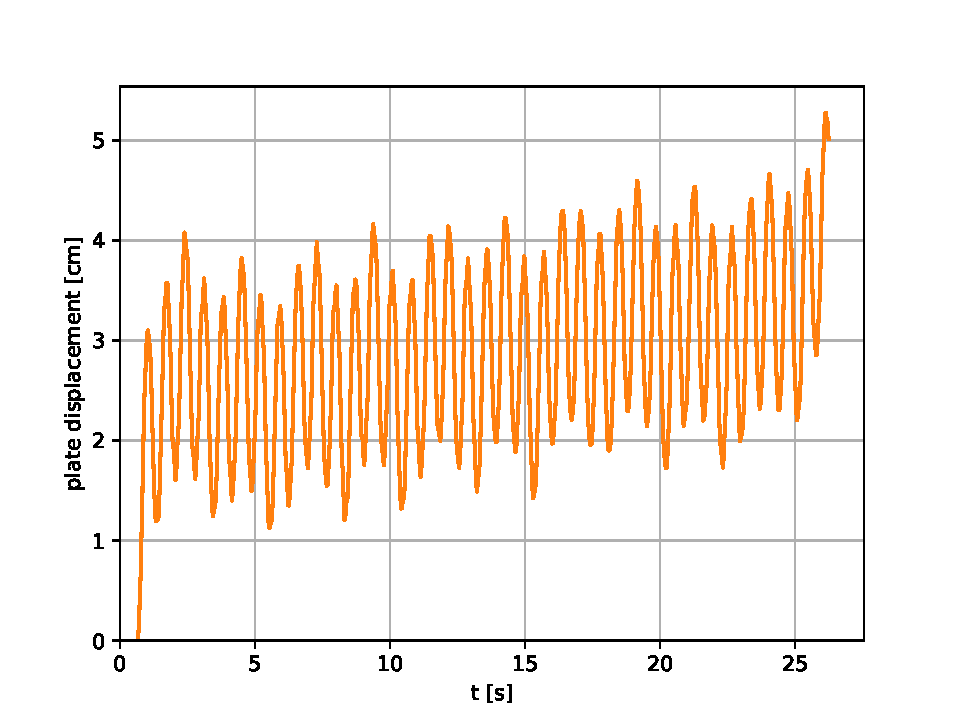
\includegraphics[width=0.45\textwidth, height=3.5cm]{graph/omega=3.00_A=2_plate.pdf}\\
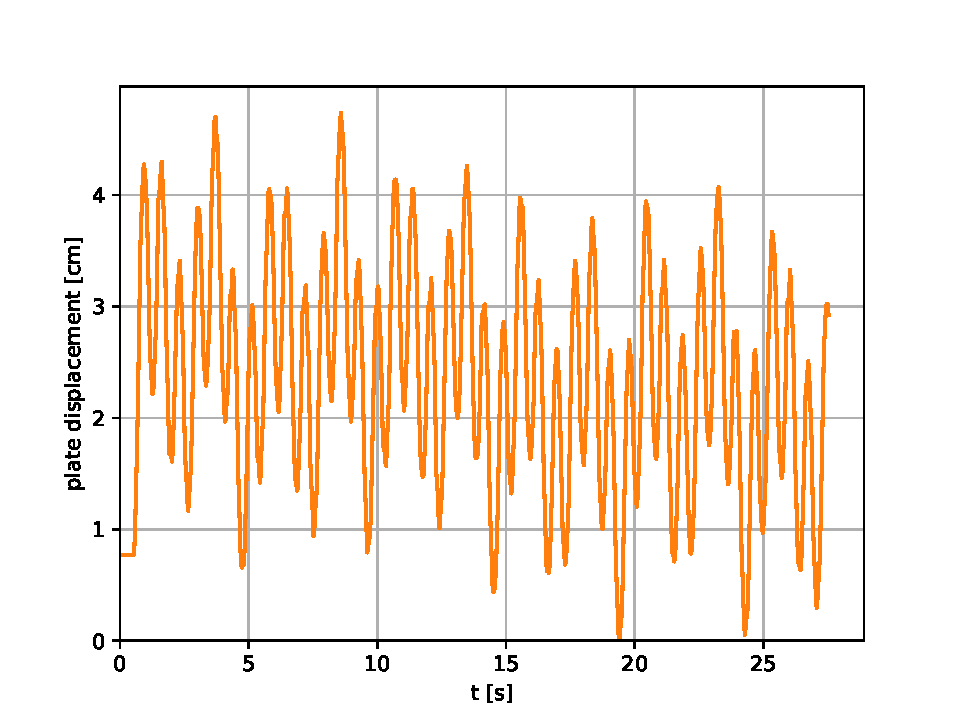
\includegraphics[width=0.45\textwidth, height=3.5cm]{graph/omega=3.00_A=3_plate.pdf}
&
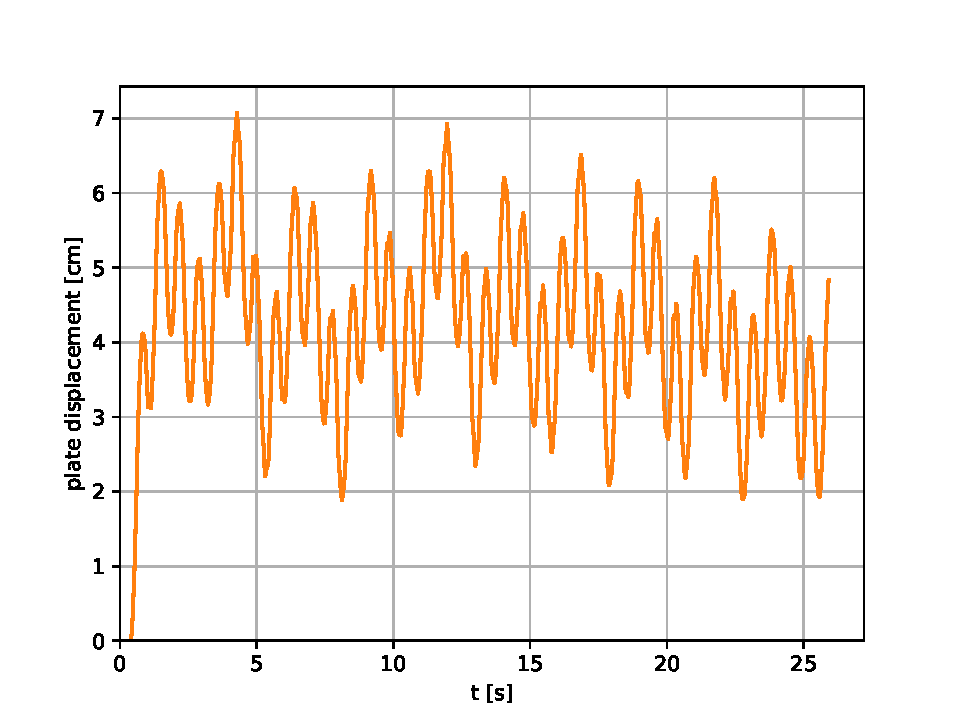
\includegraphics[width=0.45\textwidth, height=3.5cm]{graph/omega=3.00_A=4_plate.pdf}\\
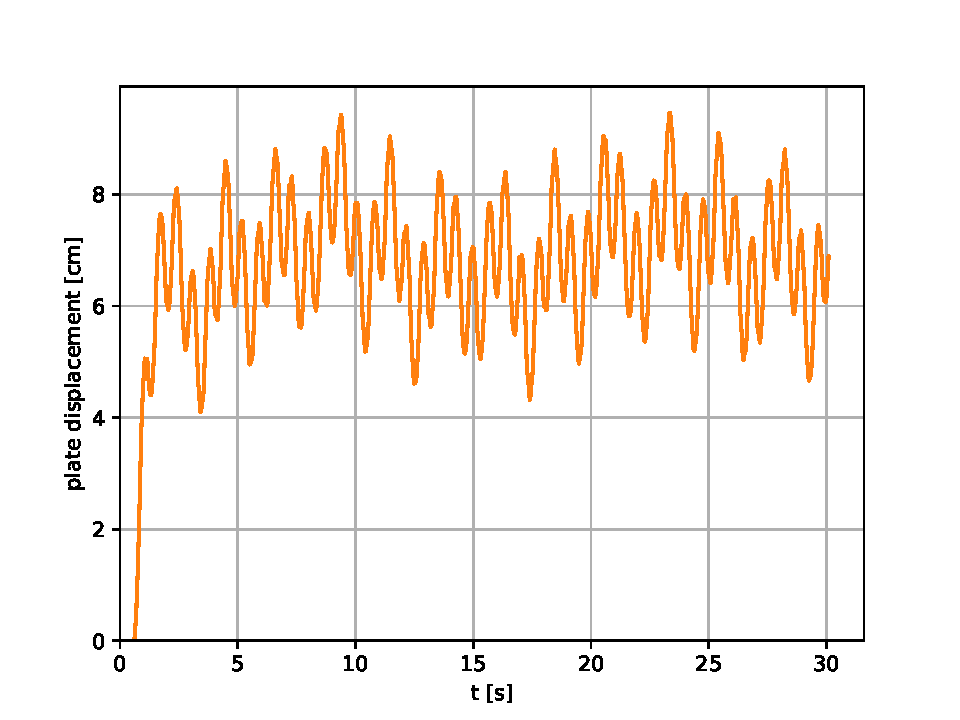
\includegraphics[width=0.45\textwidth, height=3.5cm]{graph/omega=3.00_A=5_plate.pdf}
&
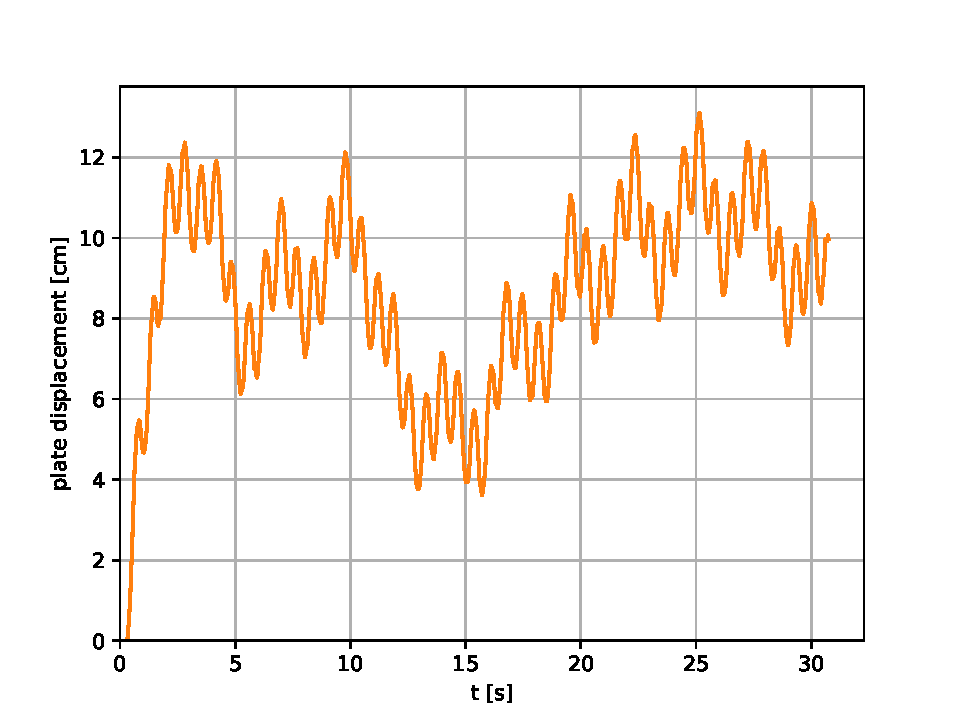
\includegraphics[width=0.45\textwidth, height=3.5cm]{graph/omega=3.00_A=6_plate.pdf}\\
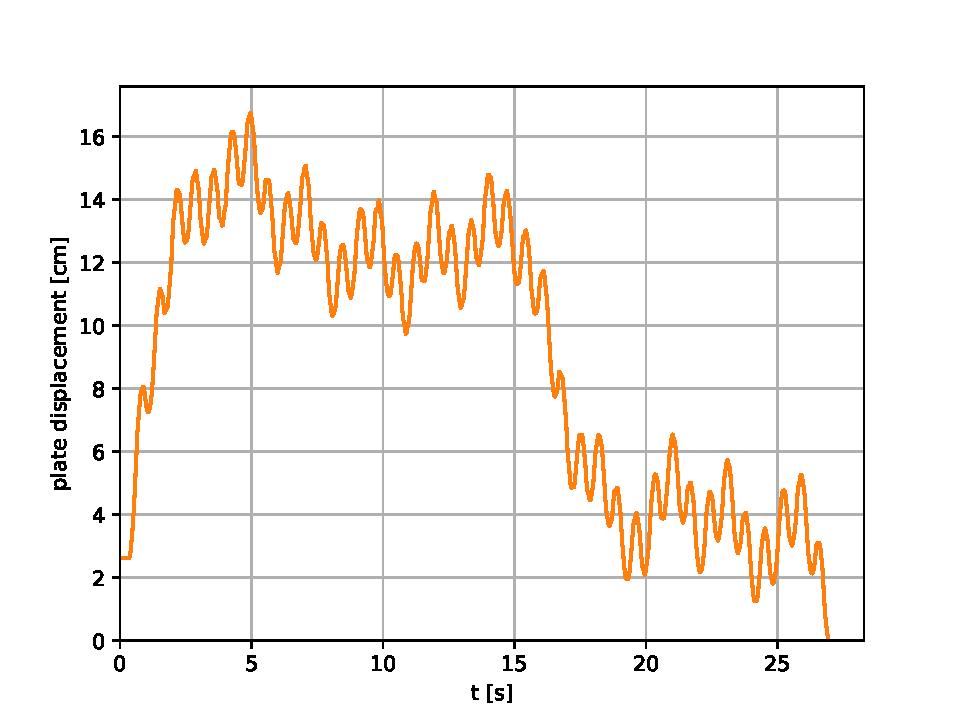
\includegraphics[width=0.45\textwidth, height=3.5cm]{graph/omega=3.00_A=7_plate.pdf}
&
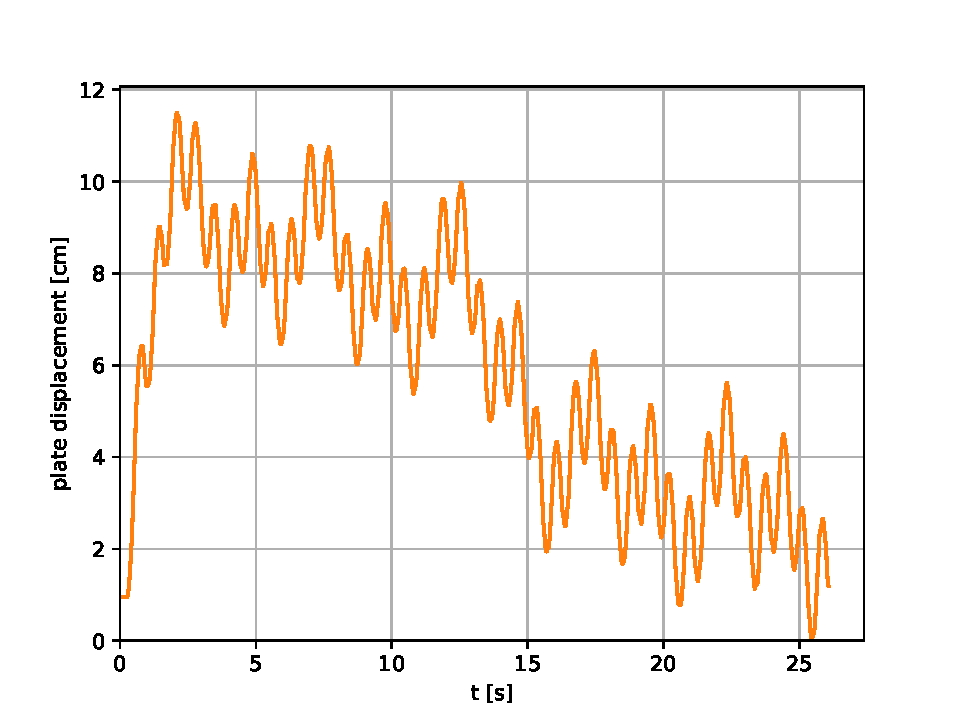
\includegraphics[width=0.45\textwidth, height=3.5cm]{graph/omega=3.00_A=8_plate.pdf}\\
\includegraphics[width=0.45\textwidth, height=3.5cm]{graph/omega=3.00_A=9_plate.pdf}
&
\includegraphics[width=0.45\textwidth, height=3.5cm]{graph/omega=3.00_A=10_plate.pdf}\\
\end{tabular}
\end{center}
\begin{tikzpicture} [remember picture, overlay]
\node at (3.9, 15.0) {(a)};
\node at (10.8, 15.0) {(b)};
\node at (3.9, 11.4) {(c)};
\node at (10.8, 11.4) {(d)};
\node at (3.9, 7.7) {(e)};
\node at (10.8, 7.7) {(f)};
\node at (3.9, 4.1) {(g)};
\node at (10.8, 4.1) {(h)};
\node at (3.9, 0.4) {(i)};
\node at (10.8, 0.4) {(j)};
\end{tikzpicture}
\caption{Plate movement - $\omega=10$ \\ (a) $A=1\mathrm{~cm}$ (b) $A=2\mathrm{~cm}$ (c) $A=3\mathrm{~cm}$ (d) $A=4\mathrm{~cm}$ (e) $A=5\mathrm{~cm}$\\(f) $A=6\mathrm{~cm}$ (g) $A=7\mathrm{~cm}$ (h) $A=8\mathrm{~cm}$ (i) $A=9\mathrm{~cm}$ (j) $A=10\mathrm{~cm}$}
\label{Data_omega=10_plate}
\end{figure}

\begin{figure}[H]
\begin{center}
\begin{tabular}{cc}
\includegraphics[width=0.45\textwidth, height=3.5cm]{graph/omega=3.50_A=1_plate.pdf}
&
\includegraphics[width=0.45\textwidth, height=3.5cm]{graph/omega=3.50_A=2_plate.pdf}\\
\includegraphics[width=0.45\textwidth, height=3.5cm]{graph/omega=3.50_A=3_plate.pdf}
&
\includegraphics[width=0.45\textwidth, height=3.5cm]{graph/omega=3.50_A=4_plate.pdf}\\
\includegraphics[width=0.45\textwidth, height=3.5cm]{graph/omega=3.50_A=5_plate.pdf}
&
\includegraphics[width=0.45\textwidth, height=3.5cm]{graph/omega=3.50_A=6_plate.pdf}\\
\includegraphics[width=0.45\textwidth, height=3.5cm]{graph/omega=3.50_A=7_plate.pdf}
&
\includegraphics[width=0.45\textwidth, height=3.5cm]{graph/omega=3.50_A=8_plate.pdf}\\
\includegraphics[width=0.45\textwidth, height=3.5cm]{graph/omega=3.50_A=9_plate.pdf}
&
\includegraphics[width=0.45\textwidth, height=3.5cm]{graph/omega=3.50_A=10_plate.pdf}\\
\end{tabular}
\end{center}
\begin{tikzpicture} [remember picture, overlay]
\node at (3.9, 15.0) {(a)};
\node at (10.8, 15.0) {(b)};
\node at (3.9, 11.4) {(c)};
\node at (10.8, 11.4) {(d)};
\node at (3.9, 7.7) {(e)};
\node at (10.8, 7.7) {(f)};
\node at (3.9, 4.1) {(g)};
\node at (10.8, 4.1) {(h)};
\node at (3.9, 0.4) {(i)};
\node at (10.8, 0.4) {(j)};
\end{tikzpicture}
\caption{Plate movement - $\omega=12$ \\ (a) $A=1\mathrm{~cm}$ (b) $A=2\mathrm{~cm}$ (c) $A=3\mathrm{~cm}$ (d) $A=4\mathrm{~cm}$ (e) $A=5\mathrm{~cm}$\\(f) $A=6\mathrm{~cm}$ (g) $A=7\mathrm{~cm}$ (h) $A=8\mathrm{~cm}$ (i) $A=9\mathrm{~cm}$ (j) $A=10\mathrm{~cm}$}
\label{Data_omega=12_plate}
\end{figure}

%%%%%%%%%%%%%%%%%%%%%%%%%%%%%%%%%%%%%%%%%%%%%%%%%%%%%%%%%%%%
\subsection{Wave height}

\begin{figure}[H]
\begin{center}
\begin{tabular}{cc}
\includegraphics[width=0.45\textwidth, height=3.5cm]{graph/omega=0.50_A=1_wave.pdf}
&
\includegraphics[width=0.45\textwidth, height=3.5cm]{graph/omega=0.50_A=2_wave.pdf}\\
\includegraphics[width=0.45\textwidth, height=3.5cm]{graph/omega=0.50_A=3_wave.pdf}
&
\includegraphics[width=0.45\textwidth, height=3.5cm]{graph/omega=0.50_A=4_wave.pdf}\\
\includegraphics[width=0.45\textwidth, height=3.5cm]{graph/omega=0.50_A=5_wave.pdf}
&
\\
&
\\
&
\\
\end{tabular}
\end{center}
\begin{tikzpicture} [remember picture, overlay]
\node at (3.9, 8.7) {(a)};
\node at (10.8, 8.7) {(b)};
\node at (3.9, 5.0) {(c)};
\node at (10.8, 5.0) {(d)};
\node at (3.9, 1.4) {(e)};
\end{tikzpicture}
\caption{Wave height - $\omega=3$ \\ (a) $A=1\mathrm{~cm}$ (b) $A=2\mathrm{~cm}$ (c) $A=3\mathrm{~cm}$ (d) $A=4\mathrm{~cm}$ (e) $A=5\mathrm{~cm}$}
\label{Data_omega=3_wave}
\end{figure}

\begin{figure}[H]
\begin{center}
\begin{tabular}{cc}
\includegraphics[width=0.45\textwidth, height=3.5cm]{graph/omega=1.00_A=1_wave.pdf}
&
\includegraphics[width=0.45\textwidth, height=3.5cm]{graph/omega=1.00_A=2_wave.pdf}\\
\includegraphics[width=0.45\textwidth, height=3.5cm]{graph/omega=1.00_A=3_wave.pdf}
&
\includegraphics[width=0.45\textwidth, height=3.5cm]{graph/omega=1.00_A=4_wave.pdf}\\
\includegraphics[width=0.45\textwidth, height=3.5cm]{graph/omega=1.00_A=5_wave.pdf}
&
\includegraphics[width=0.45\textwidth, height=3.5cm]{graph/omega=1.00_A=6_wave.pdf}\\
\includegraphics[width=0.45\textwidth, height=3.5cm]{graph/omega=1.00_A=7_wave.pdf}
&
\\
&
\\
\end{tabular}
\end{center}
\begin{tikzpicture} [remember picture, overlay]
\node at (3.9, 11.8) {(a)};
\node at (10.8, 11.8) {(b)};
\node at (3.9, 8.2) {(c)};
\node at (10.8, 8.2) {(d)};
\node at (3.9, 4.5) {(e)};
\node at (10.8, 4.5) {(f)};
\node at (3.9, 0.9) {(g)};
\end{tikzpicture}
\caption{Wave height - $\omega=4$ \\ (a) $A=1\mathrm{~cm}$ (b) $A=2\mathrm{~cm}$ (c) $A=3\mathrm{~cm}$ (d) $A=4\mathrm{~cm}$ (e) $A=5\mathrm{~cm}$\\ (f) $A=6\mathrm{~cm}$ (g) $A=7\mathrm{~cm}$}
\label{Data_omega=4_wave}
\end{figure}

\begin{figure}[H]
\begin{center}
\begin{tabular}{cc}
\includegraphics[width=0.45\textwidth, height=3.5cm]{graph/omega=1.50_A=1_wave.pdf}
&
\includegraphics[width=0.45\textwidth, height=3.5cm]{graph/omega=1.50_A=2_wave.pdf}\\
\includegraphics[width=0.45\textwidth, height=3.5cm]{graph/omega=1.50_A=3_wave.pdf}
&
\includegraphics[width=0.45\textwidth, height=3.5cm]{graph/omega=1.50_A=4_wave.pdf}\\
\includegraphics[width=0.45\textwidth, height=3.5cm]{graph/omega=1.50_A=5_wave.pdf}
&
\includegraphics[width=0.45\textwidth, height=3.5cm]{graph/omega=1.50_A=6_wave.pdf}\\
\includegraphics[width=0.45\textwidth, height=3.5cm]{graph/omega=1.50_A=7_wave.pdf}
&
\includegraphics[width=0.45\textwidth, height=3.5cm]{graph/omega=1.50_A=8_wave.pdf}\\
\includegraphics[width=0.45\textwidth, height=3.5cm]{graph/omega=1.50_A=9_wave.pdf}
&
\includegraphics[width=0.45\textwidth, height=3.5cm]{graph/omega=1.50_A=10_wave.pdf}\\
\end{tabular}
\end{center}
\begin{tikzpicture} [remember picture, overlay]
\node at (3.9, 15.0) {(a)};
\node at (10.8, 15.0) {(b)};
\node at (3.9, 11.4) {(c)};
\node at (10.8, 11.4) {(d)};
\node at (3.9, 7.7) {(e)};
\node at (10.8, 7.7) {(f)};
\node at (3.9, 4.1) {(g)};
\node at (10.8, 4.1) {(h)};
\node at (3.9, 0.4) {(i)};
\node at (10.8, 0.4) {(j)};
\end{tikzpicture}
\caption{Wave height - $\omega=6$ \\ (a) $A=1\mathrm{~cm}$ (b) $A=2\mathrm{~cm}$ (c) $A=3\mathrm{~cm}$ (d) $A=4\mathrm{~cm}$ (e) $A=5\mathrm{~cm}$\\(f) $A=6\mathrm{~cm}$ (g) $A=7\mathrm{~cm}$ (h) $A=8\mathrm{~cm}$ (i) $A=9\mathrm{~cm}$ (j) $A=10\mathrm{~cm}$}
\label{Data_omega=6_wave}
\end{figure}

\begin{figure}[H]
\begin{center}
\begin{tabular}{cc}
\includegraphics[width=0.45\textwidth, height=3.5cm]{graph/omega=2.00_A=1_wave.pdf}
&
\includegraphics[width=0.45\textwidth, height=3.5cm]{graph/omega=2.00_A=2_wave.pdf}\\
\includegraphics[width=0.45\textwidth, height=3.5cm]{graph/omega=2.00_A=3_wave.pdf}
&
\includegraphics[width=0.45\textwidth, height=3.5cm]{graph/omega=2.00_A=4_wave.pdf}\\
\includegraphics[width=0.45\textwidth, height=3.5cm]{graph/omega=2.00_A=5_wave.pdf}
&
\includegraphics[width=0.45\textwidth, height=3.5cm]{graph/omega=2.00_A=6_wave.pdf}\\
\includegraphics[width=0.45\textwidth, height=3.5cm]{graph/omega=2.00_A=7_wave.pdf}
&
\includegraphics[width=0.45\textwidth, height=3.5cm]{graph/omega=2.00_A=8_wave.pdf}\\
\includegraphics[width=0.45\textwidth, height=3.5cm]{graph/omega=2.00_A=9_wave.pdf}
&
\includegraphics[width=0.45\textwidth, height=3.5cm]{graph/omega=2.00_A=10_wave.pdf}\\
\end{tabular}
\end{center}
\begin{tikzpicture} [remember picture, overlay]
\node at (3.9, 15.0) {(a)};
\node at (10.8, 15.0) {(b)};
\node at (3.9, 11.4) {(c)};
\node at (10.8, 11.4) {(d)};
\node at (3.9, 7.7) {(e)};
\node at (10.8, 7.7) {(f)};
\node at (3.9, 4.1) {(g)};
\node at (10.8, 4.1) {(h)};
\node at (3.9, 0.4) {(i)};
\node at (10.8, 0.4) {(j)};
\end{tikzpicture}
\caption{Wave height - $\omega=7$ \\ (a) $A=1\mathrm{~cm}$ (b) $A=2\mathrm{~cm}$ (c) $A=3\mathrm{~cm}$ (d) $A=4\mathrm{~cm}$ (e) $A=5\mathrm{~cm}$\\(f) $A=6\mathrm{~cm}$ (g) $A=7\mathrm{~cm}$ (h) $A=8\mathrm{~cm}$ (i) $A=9\mathrm{~cm}$ (j) $A=10\mathrm{~cm}$}
\label{Data_omega=7_wave}
\end{figure}

\begin{figure}[H]
\begin{center}
\begin{tabular}{cc}
\includegraphics[width=0.45\textwidth, height=3.5cm]{graph/omega=2.50_A=1_wave.pdf}
&
\includegraphics[width=0.45\textwidth, height=3.5cm]{graph/omega=2.50_A=2_wave.pdf}\\
\includegraphics[width=0.45\textwidth, height=3.5cm]{graph/omega=2.50_A=3_wave.pdf}
&
\includegraphics[width=0.45\textwidth, height=3.5cm]{graph/omega=2.50_A=4_wave.pdf}\\
\includegraphics[width=0.45\textwidth, height=3.5cm]{graph/omega=2.50_A=5_wave.pdf}
&
\includegraphics[width=0.45\textwidth, height=3.5cm]{graph/omega=2.50_A=6_wave.pdf}\\
\includegraphics[width=0.45\textwidth, height=3.5cm]{graph/omega=2.50_A=7_wave.pdf}
&
\includegraphics[width=0.45\textwidth, height=3.5cm]{graph/omega=2.50_A=8_wave.pdf}\\
\includegraphics[width=0.45\textwidth, height=3.5cm]{graph/omega=2.50_A=9_wave.pdf}
&
\includegraphics[width=0.45\textwidth, height=3.5cm]{graph/omega=2.50_A=10_wave.pdf}\\
\end{tabular}
\end{center}
\begin{tikzpicture} [remember picture, overlay]
\node at (3.9, 15.0) {(a)};
\node at (10.8, 15.0) {(b)};
\node at (3.9, 11.4) {(c)};
\node at (10.8, 11.4) {(d)};
\node at (3.9, 7.7) {(e)};
\node at (10.8, 7.7) {(f)};
\node at (3.9, 4.1) {(g)};
\node at (10.8, 4.1) {(h)};
\node at (3.9, 0.4) {(i)};
\node at (10.8, 0.4) {(j)};
\end{tikzpicture}
\caption{Wave height - $\omega=9$ \\ (a) $A=1\mathrm{~cm}$ (b) $A=2\mathrm{~cm}$ (c) $A=3\mathrm{~cm}$ (d) $A=4\mathrm{~cm}$ (e) $A=5\mathrm{~cm}$\\(f) $A=6\mathrm{~cm}$ (g) $A=7\mathrm{~cm}$ (h) $A=8\mathrm{~cm}$ (i) $A=9\mathrm{~cm}$ (j) $A=10\mathrm{~cm}$}
\label{Data_omega=9_wave}
\end{figure}

\begin{figure}[H]
\begin{center}
\begin{tabular}{cc}
\includegraphics[width=0.45\textwidth, height=3.5cm]{graph/omega=3.00_A=1_wave.pdf}
&
\includegraphics[width=0.45\textwidth, height=3.5cm]{graph/omega=3.00_A=2_wave.pdf}\\
\includegraphics[width=0.45\textwidth, height=3.5cm]{graph/omega=3.00_A=3_wave.pdf}
&
\includegraphics[width=0.45\textwidth, height=3.5cm]{graph/omega=3.00_A=4_wave.pdf}\\
\includegraphics[width=0.45\textwidth, height=3.5cm]{graph/omega=3.00_A=5_wave.pdf}
&
\includegraphics[width=0.45\textwidth, height=3.5cm]{graph/omega=3.00_A=6_wave.pdf}\\
\includegraphics[width=0.45\textwidth, height=3.5cm]{graph/omega=3.00_A=7_wave.pdf}
&
\includegraphics[width=0.45\textwidth, height=3.5cm]{graph/omega=3.00_A=8_wave.pdf}\\
\includegraphics[width=0.45\textwidth, height=3.5cm]{graph/omega=3.00_A=9_wave.pdf}
&
\includegraphics[width=0.45\textwidth, height=3.5cm]{graph/omega=3.00_A=10_wave.pdf}\\
\end{tabular}
\end{center}
\begin{tikzpicture} [remember picture, overlay]
\node at (3.9, 15.0) {(a)};
\node at (10.8, 15.0) {(b)};
\node at (3.9, 11.4) {(c)};
\node at (10.8, 11.4) {(d)};
\node at (3.9, 7.7) {(e)};
\node at (10.8, 7.7) {(f)};
\node at (3.9, 4.1) {(g)};
\node at (10.8, 4.1) {(h)};
\node at (3.9, 0.4) {(i)};
\node at (10.8, 0.4) {(j)};
\end{tikzpicture}
\caption{Wave height - $\omega=10$ \\ (a) $A=1\mathrm{~cm}$ (b) $A=2\mathrm{~cm}$ (c) $A=3\mathrm{~cm}$ (d) $A=4\mathrm{~cm}$ (e) $A=5\mathrm{~cm}$\\(f) $A=6\mathrm{~cm}$ (g) $A=7\mathrm{~cm}$ (h) $A=8\mathrm{~cm}$ (i) $A=9\mathrm{~cm}$ (j) $A=10\mathrm{~cm}$}
\label{Data_omega=10_wave}
\end{figure}

\begin{figure}[H]
\begin{center}
\begin{tabular}{cc}
\includegraphics[width=0.45\textwidth, height=3.5cm]{graph/omega=3.50_A=1_wave.pdf}
&
\includegraphics[width=0.45\textwidth, height=3.5cm]{graph/omega=3.50_A=2_wave.pdf}\\
\includegraphics[width=0.45\textwidth, height=3.5cm]{graph/omega=3.50_A=3_wave.pdf}
&
\includegraphics[width=0.45\textwidth, height=3.5cm]{graph/omega=3.50_A=4_wave.pdf}\\
\includegraphics[width=0.45\textwidth, height=3.5cm]{graph/omega=3.50_A=5_wave.pdf}
&
\includegraphics[width=0.45\textwidth, height=3.5cm]{graph/omega=3.50_A=6_wave.pdf}\\
\includegraphics[width=0.45\textwidth, height=3.5cm]{graph/omega=3.50_A=7_wave.pdf}
&
\includegraphics[width=0.45\textwidth, height=3.5cm]{graph/omega=3.50_A=8_wave.pdf}\\
\includegraphics[width=0.45\textwidth, height=3.5cm]{graph/omega=3.50_A=9_wave.pdf}
&
\includegraphics[width=0.45\textwidth, height=3.5cm]{graph/omega=3.50_A=10_wave.pdf}\\
\end{tabular}
\end{center}
\begin{tikzpicture} [remember picture, overlay]
\node at (3.9, 15.0) {(a)};
\node at (10.8, 15.0) {(b)};
\node at (3.9, 11.4) {(c)};
\node at (10.8, 11.4) {(d)};
\node at (3.9, 7.7) {(e)};
\node at (10.8, 7.7) {(f)};
\node at (3.9, 4.1) {(g)};
\node at (10.8, 4.1) {(h)};
\node at (3.9, 0.4) {(i)};
\node at (10.8, 0.4) {(j)};
\end{tikzpicture}
\caption{Wave height - $\omega=12$ \\ (a) $A=1\mathrm{~cm}$ (b) $A=2\mathrm{~cm}$ (c) $A=3\mathrm{~cm}$ (d) $A=4\mathrm{~cm}$ (e) $A=5\mathrm{~cm}$\\(f) $A=6\mathrm{~cm}$ (g) $A=7\mathrm{~cm}$ (h) $A=8\mathrm{~cm}$ (i) $A=9\mathrm{~cm}$ (j) $A=10\mathrm{~cm}$}
\label{Data_omega=12_wave}
\end{figure}